\documentclass[9pt,twocolumn,twoside]{pnas-new}
% Use the lineno option to display guide line numbers if required.
% Note that the use of elements such as single-column equations
% may affect the guide line number alignment.
\templatetype{pnasresearcharticle} % Choose template
% {pnasresearcharticle} = Template for a two-column research article
% {pnasmathematics} = Template for a one-column mathematics article
% {pnasinvited} = Template for a PNAS invited submission
%\usepackage{graphicx}

\usepackage{amsmath,amsfonts,amssymb}
\usepackage{fullpage}
\usepackage{color}
\usepackage{bm}
\newcommand{\rr}[1]{{\rm #1}}



% \usepackage[english]{babel}
% \usepackage[latin1]{inputenc}
% \usepackage[T1]{fontenc}
% \usepackage{color}
% \usepackage{float}
% \usepackage{verbatim}
% \usepackage{graphicx}
% \usepackage{bm}
% \usepackage{mathtools}
% \usepackage{stmaryrd}
% \usepackage{anyfontsize}
% \usepackage{fullpage}
% \usepackage{color}


% \graphicspath{{../Enigma/figures/}}
\definecolor{darkblue}{rgb}{0,0,0.6}
\definecolor{darkcyan}{rgb}{0.1,0.3,0.4}
\definecolor{darkgreen}{rgb}{0,0.4,0}
\definecolor{darkred}{rgb}{0.6,0,0}
\newcommand{\jy}[1]{\textcolor{darkblue}{#1}}

% \title{Quantization of ecological interactions yields insights into ecosystem assembly and dynamics}
\title{Diverse interactions and ecosystem engineering stabilize community assembly}

% Use letters for affiliations, numbers to show equal authorship (if applicable) and to indicate the corresponding author
\author[a,b,1]{Justin D. Yeakel}
% \author[a,b]{Hattie}
\author[c]{Mathias M. Pires}
\author[c]{Marcus A. M. de Aguiar}
\author[d]{James L. O'Donnell}
\author[e]{Paulo R. Guimar\~aes Jr.}
\author[f]{Dominique Gravel}
\author[g]{Thilo Gross}


\affil[a]{School of Natural Sciences, University of California Merced, Merced, CA 95343, USA}
\affil[b]{Santa Fe Institute}
\affil[c]{Universidade Estadual de Campinas}
\affil[d]{University of Washington}
\affil[e]{Universidade de S\~ao Paulo}
\affil[f]{Universit\`e de Sherbrooke}
\affil[g]{University of California Davis, Davis CA}

% Please give the surname of the lead author for the running footer
\leadauthor{Yeakel}

% Please add here a significance statement to explain the relevance of your work
\vspace{-3mm}
\significancestatement{
Community assembly is constrained by interactions between and among species, many of which can have lasting effects on the environment. We explore the influence of these ecosystem engineers on colonization and extinction dynamics using a network model that includes trophic, mutualistic, and engineering dependencies between species and the abiotic environment. We find that ecosystem engineering can stabilize assembly particularly when multiple engineers have similar effects on the community.
%Authors must submit a 120-word maximum statement about the significance of their research paper written at a level understandable to an undergraduate educated scientist outside their field of speciality. The primary goal of the Significance Statement is to explain the relevance of the work in broad context to a broad readership. The Significance Statement appears in the paper itself and is required for all research papers.
}

% Please include corresponding author, author contribution and author declaration information
\authorcontributions{JDY and TG conceived of the model framework. JDY, MMP, MAMA, and TG designed the analyses. JDY, MMP, MAMA, JLOD, PRG, DG, and TG analyzed the results and contributed to multiple versions of the manuscript.}
\authordeclaration{The authors declare no conflict of interest}
\correspondingauthor{\textsuperscript{1}To whom correspondence should be addressed. E-mail: jyeakel@ucmerced.edu}

% Keywords are not mandatory, but authors are strongly encouraged to provide them. If provided, please include two to five keywords, separated by the pipe symbol, e.g:
\keywords{Ecological networks $|$ Community assembly $|$ Ecosystem engineering $|$ Niche construction $|$ Extinction}
\begin{abstract}
The complexity of an ecological community can be distilled into a network, where diverse interactions connect species in a web of dependencies. Species interact not only with each other but indirectly through environmental effects, however the role of these ecosystem engineers has not yet been considered in models of ecological networks. Here we explore the dynamics of ecosystem assembly, where the colonization and extinction of species within a community depends on the constraints imposed by trophic, service, and engineering dependencies. We show that our assembly model reproduces many key features of ecological systems, such as the role of generalists during assembly, realistic maximum trophic levels, and increased nestedness with higher frequencies of mutualisms. We find that ecosystem engineering has large and nonlinear effects on extinction rates, facilitating robustness by creating niche space, but at the same time increasing the magnitude of extinction cascades. We emphasize the importance of redundancies in engineered effects and show that such redundancy lowers the barriers to colonization, promoting community diversity. Together, our results suggest that ecological engineers may enhance community diversity while increasing persistence by facilitating colonization and limiting competitive exclusion. 
% First, we show that the assembly of species networks in the absence of engineering reproduces many features observed in empirical systems.
% These include changes in the proportion of generalists over the course of assembly that accord with measured data, and trophic diversity similar to empirical observations. % both maximum trophic level and 
% Second, we show that increasing the frequency of mutualistic interactions leads to the assembly of ecological networks that are more nested, a hallmark feature of mutualistic systems \cite{Bascompte2003}.
% We next explore the effects of ecosystem engineering on the dynamics of community assembly.
% Our third key result shows that increasing both the number of ecosystem engineers and engineering interactions within a community has nonlinear effects on observed extinction rates.
% While we find that a low amount of engineering increases extinction rates, a high amount of engineering serves to reduce extinction rates due to the large niche space facilitated by engineers.
% Finally, we show that the inclusion of engineering modifies the effects of mutualistic interactions, and can reduce the negative effects that mutualisms have on species' persistence.
\end{abstract}
\dates{This manuscript was compiled on \today}
\doi{\url{www.pnas.org/cgi/doi/10.1073/pnas.XXXXXXXXXX}}



\begin{document}
% Optional adjustment to line up main text (after abstract) of first page with line numbers, when using both lineno and twocolumn options.
% You should only change this length when you've finalised the article contents.
\verticaladjustment{-2pt}

\maketitle
\thispagestyle{firststyle}
\ifthenelse{\boolean{shortarticle}}{\ifthenelse{\boolean{singlecolumn}}{\abscontentformatted}{\abscontent}}{}


%structure is the result of dynamics
To unravel nature's secrets we must simplify its abundant complexities and idiosyncrasies.
% Simplifying the abundant complexities and eccentricities of nature is necessary to unravel its secrets.
The layers of natural history giving rise to an ecological community can be distilled -- among many forms -- into a network, where nodes represent species and links represent interactions between them.
Networks are generally constructed for one type of interaction, such as food webs capturing predation \cite{Paine1966,Dunne2002,Pascual2006} or pollination networks capturing a specific mutualistic interaction \cite{Bascompte2013}, and continues to lead to significant breakthroughs in our understanding of the dynamical consequences of community structure \cite{May1972,Gross2009,Allesina2012}, assembly \cite{Ponisio2017}, and coevolution \cite{Guimaraes2017}. 
Recent interest in `multilayer networks' comprising multiple interaction types (multitype interactions) may provide additional insight into these processes \cite{Kefi2016,Pilosof2017}. 
However, interactions where species affect others by altering the environment in a lasting way have not yet been incorporated into models of ecological networks. 
These interactions, known as ecosystem engineering \cite{Lawton1994,OdlingSmee2013} or more generally niche construction \cite{OdlingSmee2013b,Fukami2015}, are quite common in nature and exist in almost every ecosystem.

% This minimalist perspective provides insight into community structure \cite{Dunne2002,Pascual2006}, and consequently, the dynamics of populations and system stability \cite{May1972,Gross2009,Allesina2012}.
% Community structure can directly impact the ability of the system to absorb external perturbations \cite{Novak2011,Aufderheide2013,Novak2016}, the existence and ubiquity of tipping points marking sudden changes in species' populations \cite{Lade2011,Boettiger2012}, and promote or inhibit extinction cascades \cite{Stouffer2011,Yeakel2014}.
% Importantly, community structure is the result of a dynamical process that takes place over time, where species are added to or removed from the community in succession \cite{Weiher2001}.
% This process is generally referred to as community assembly, and though it is an engine for much that we observe in nature, is not well understood.

%multiple interaction types
% Ecological networks are generally constructed and analyzed with respect to a single type of interaction.
% For example, beneficial relationships between species form the foundation of mutualistic networks, whereas antagonistic interactions form the foundation of trophic networks, or food webs. %- which are often trophic in one direction and a reproductive service in the other -
% There has been a growing interest in understanding community structure by taking into account diverse interaction types \cite{Kefi2016}, where multiple unique interactions are included, sometimes in a multi-layer network \cite{Pilosof2017}.
% Interactions between two species are inherently compound in nature, such that both species in an interaction experiences different effects.
% For example, mutualistic interactions generally involve a flow of biomass in one direction and a reproductive service in the other; in a trophic interaction there is a flow of biomass from the prey to the predator but not the reverse.
% This asymmetry is generally encoded into the dynamics, rather than the network structure itself \cite{Gross2009,Allesina2012}.


%Ecosystem engineering
Diverse interactions occur not only between species but indirectly through the effects that species have on their environment \cite{Jones1994,Olff2009,OdlingSmee2013}.
Elephants root out large saplings and small trees, enabling the formation and maintenance of grasslands \cite{Haynes2012} and creating habitat for smaller vertebrates \cite{Pringle2008}.
Burrowing rodents create shelter and promote primary production by aerating the soil \cite{Reichman2002}, salmon and aquatic invertebrates create freshwater habitats by changing stream morphology \cite{Moore2006}, and leaf-cutter ants alter microclimates, influencing seedling survival and plant growth \cite{Meyer2011}.
These examples illustrate ecosystem engineering, where the engineering organism alters the environment on timescales longer than its own \cite{Hastings2007}.

% On ecological timescales, ecosystem engineers are relatively common and can alter the landscape on which ecological interactions occur \cite{Wright2006}.

Ecosystem engineering not only impacts communities on ecological timescales, but has profoundly shaped the evolution of life on Earth \cite{Erwin2008}.
For example, the emergence of multicellular cyanobacteria fundamentally altered the atmosphere during the Great Oxidation Event of the Proterozoic roughly 2.5 Byrs BP \cite{Erwin2008,Schirrmeister2013}, paving the way for the biological invasion of terrestrial habitats.
In the oceans it is thought that rRNA and protein biogenesis of aquatic photoautotrophs drove the nitrogen:phosphorous ratio (the Redfield Ratio) to ca. 16:1 matching that of plankton \cite{Loladze2011}, illustrating that engineering clades can have much larger, sometimes global-scale effects.
% While local habitats can be significantly impacted by single engineering species, larger scale effects are generally modified by diverse engineering clades.
% While engineering species such as elephants can have considerable impact on local environments, 
% which illustrates that engineering clades can have much larger, sometimes global-scale effects.


% These example describe indirect interactions between ecosystem engineers and species that rely on their engineering, through an environmental intermediary.
% By way of their indirectness, these interactions are difficult to document.

% GLOBAL SHIFTS ORIGINATE DUE TO ENGINEERING BY A LARGE GROUP OF RELATED SPECIES


% 
% Recent efforts have examined engineering through the lens of niche construction \cite{Krakauer2009}, such as the construction of shared resources such as metabolite in microbiotic communities \cite{Kallus2017}.
% Engineering by way of niche construction is a strategy that may be evolutionary precarious \cite{Krakauer2009}, but may also serve as the missing ingredient that stabilizing some complex ecological systems \cite{Muscarella2017}.

%NOTE: From THILO
% The effect of the abiotic environemt on the lifeforms is commonly included in models because it is felt to be important and can (at least to first approximation) be easily systematized. By compaison the way in which species engineer the environment defies easy systemization due to the multitude of mechanisms by which the engineering occurs. Despite being perhaps of equal importnace engineering is hence omitted from most models. 



The effect of the environment on species is commonly included in models of ecological dynamics \cite{Woodward2010,Brose2012,Gibert2019b} due to its acknowledged importance and because it can -- to first approximation -- be easily systematized. 
By comparison the way in which species engineer the environment defies easy systemization due to the multitude of mechanisms by which engineering occurs.
% Despite its relevance, the interactions facilitated by ecosystem engineers have not been included in models of ecological networks.
% Interactions between species and the abiotic environment have been conceptually described \cite{Olff2009,Getz2011}, however how these effects impact community function has not been explored.
While interactions between species and the abiotic environment have been conceptually described \cite{Olff2009,Getz2011}, the absence of engineered effects in network models was addressed by Odling-Smee et al. \cite{OdlingSmee2013}, where they outlined a conceptual framework that included both species and abiotic compartments as nodes of a network, with links denoting both biotic and abiotic interactions.
% Importantly, they emphasize the potential eco-evolutionary consequences of prior alterations to the environment influencing an ecological system at some future state.

% Here we model the assembly of ecological communities by the successive arrival of new entities from a source pool into an initially empty system. 
% These entities are modeled as nodes of a network, which include

%HERE WE...
Here we model the assembly of an ecological network where nodes represent ecological entities, including engineering species, non-engineering species, and the effects of the former on the environment, which we call abiotic \emph{modifiers}.
The links of the network that connect both species and modifiers represent trophic (\emph{eat} interactions), service (\emph{need} interactions), and engineering dependencies, respectively (Fig. \ref{fig:model}; see Materials and Methods for a full description).
Trophic interactions represent both predation as well as parasitism, whereas service interactions account for all non-trophic interactions such as pollination or seed dispersal.
In our framework a traditional mutualism (such as a plant-pollinator interaction) consists of a service (need) interaction in one direction and a trophic (eat) interaction in the other.
These multitype interactions between species and modifiers thus embed multiple dependent ecological sub-systems into a single network (Fig. \ref{fig:model}). % with interactions formed by the pairing of two dependency types (eat, need, make;
Modifiers in our framework overlap conceptually with the `abiotic compartments' described in Odling-Smee et al. \cite{OdlingSmee2013}.
Following Pillai et al. \cite{Pillai2011}, we do not track the abundances of biotic or abiotic entities but only track their presence or absence.
We use this framework to explore the dynamics of ecosystem assembly, where the colonization and extinction of species within a community depends on the constraints imposed by the trophic, service, and engineering dependencies.
We then show how observed network structures emerge from the process of assembly, compare their attributes with those from empirical systems, and examine the effects of ecosystem engineers.
% Because ecological assembly is not a memory-less process, it is likely that engineers can have considerable impact on the emergence of community structure and dynamics.
% We use this general framework to study community assembly by invasion of species and their abiotic modifiers, taking into account how interactions between them drive both colonization and extinction.
% Second we integrate the dynamics of invasion of multiple species and abiotic factors with network theory and show how observed network structures depend on historical contingencies. 

Our results offer four key insights into the roles of multitype interactions and ecosystem engineering in driving community assembly.
First, we show that the assembly of communities in the absence of engineering reproduces many features observed in empirical systems.
These include changes in the proportion of generalists over the course of assembly that accord with measured data and trophic diversity similar to empirical observations. % both maximum trophic level and 
Second, we show that increasing the frequency of mutualistic interactions leads to the assembly of ecological networks that are more nested, a common feature of diverse mutualistic systems \cite{Bascompte2003}, but are also less robust.
% We next explore the effects of ecosystem engineering on the dynamics of community assembly.
Our third key result shows that increasing the proportion of ecosystem engineers within a community has nonlinear effects on observed extinction rates.
While we find that a low amount of engineering increases extinction rates, a high amount of engineering has the opposite effect.
% We find that the role of mutualisms on community robustness is linked to the frequency of engineers
% In systems that are highly engineered, the negative effects of mutualisms are reduced
% , and that the inclusion of engineering modifies the effects of service interactions.
Finally we show that redundancies in engineered effects promote community diversity by lowering the barriers to colonization.\\
%and can reduce the negative effects that mutualisms have on species' persistence.
% Only by understanding the effects of engineers on communities can we gain insight into 

% However, we also observe that increased mutualistic dependencies in the assembled communities lower species' persistence.
% This suggests that while nested mutualistic networks appear to be dynamically favored (cf. Ref. \citenum{Rohr2014}), our model predicts that the additional inter-dependencies associated mutualisms should will lead to greater species turnover and changes in community composition.

% 
% %Model description: Pool, colonization, extinction (interaction strength), modifiers
% \noindent \textbf{Assembly of the ENIgMa network}\\
% A combination of two directional interactions between a pair of species defines the ecological relationship linking both.
% % As such, the trophic and mutualistic interactions mentioned above can be deconstructed into two directional interactions.
% A mutualistic interaction between plant x and pollinator y can thus be deconstructed into an `eat' interaction from species x to y and a \emph{need} interaction from species y to x.
% The former represents a directional trophic interaction, or a resource dependency, whereas the latter represents a reproductive service, or a dependency that does not involve biomass flow.
% Another type of mutualism is one defined by non-resource dependencies for both species, often called a service-service mutualism.
% In this case, each species would be connected to the other by directional \emph{need} interactions.
% A trophic interaction between species x and y can be deconstructed by an \emph{eat} interaction from the consumer x to the prey y, but the absence of an interaction from prey y to the consumer x, as the prey does not interact meaningfully with the consumer.
% Some species pairs may participate in bi-directional trophic interactions, where the consumer/resource role changes over the course of each species' life history.
% In this case, each species would be connected to the other by directional \emph{eat} interactions.
% 
% 
% %Interactions with both species and the environment (engineering)
% Ecosystem engineering can be formalized by the creation of a modifier by an engineering species that can be interacted with by other members of a community.
% modifiers made by ecosystem engineers represent any alteration made to the environment, whether this be changes to the stoichiometry of the atmosphere (e.g. primary producers; refs), physical modifications to the landscape (e.g. beavers, salmon; refs), or the production of unique habitats for other organisms (e.g. tree trunks; refs).
% modifiers can be represented in ecological network alongside species as nodes, but where they must be connected to engineering species by a \emph{make} interaction.
% The \emph{make} interaction between an engineering species and the engineered modifier denotes the dependency of the environmental effect on the effector.
% 


%Food webs
\vspace{-3mm}
\noindent \textbf{Assembly without ecosystem engineering}\\
\noindent Communities assemble by random colonization from a source pool.
A species from the source pool can colonize if it finds at least one resource that it can consume (one \emph{eat} interaction is satisfied; cf. Ref. \citenum{Gravel2011}) and all of its non-trophic needs are met (all \emph{need} interactions are satisfied). 
% Colonization is possible if a species can fulfill $\geq 1$ trophic requirement (cf. Ref. \citenum{Gravel2011}) and \emph{all} of its service requirements.
As such, the service interactions are assumed to be obligate, whereas trophic interactions are flexible.
Following the establishment of an autotrophic base, the arrival of mixotrophs and lower trophic heterotrophs create opportunities for organisms occupying higher trophic levels to invade.
This expanding niche space initially serves as an accelerator for community growth.
 % comprise the initial colonizers, succeeded by higher trophic consumers.
% Interestingly, we find that community growth is diversity dependent and appears logistic, where the initial colonization phase appears exponential.

Following the initial colonization phase, extinctions begin to slow the rate of community growth.
Primary extinctions occur by the competitive exclusion of species sharing similar resources.
A species' competition strength is determined by its interactions: competition strength is enhanced by the number of need interactions and penalized by its trophic generality (number of prey) and vulnerability (number of predators).
Secondary extinctions occur when species lose its last trophic or any of its service requirements.
See Fig. \ref{fig:model}D,~E for an illustration of the assembly process. 
As the colonization and extinction rates converge, the community reaches a steady state around which it oscillates (Fig. \ref{fig:trophic}A).
See Materials and Methods and Supporting Information, section I for a complete description of the assembly process. % due to losses from primary extinctions.
% As species richness increases, competitive exclusion initiates the extinction process, followed by secondary extinctions due to the loss of trophic and service requirements among species.


\begin{figure}[h!]
\centering
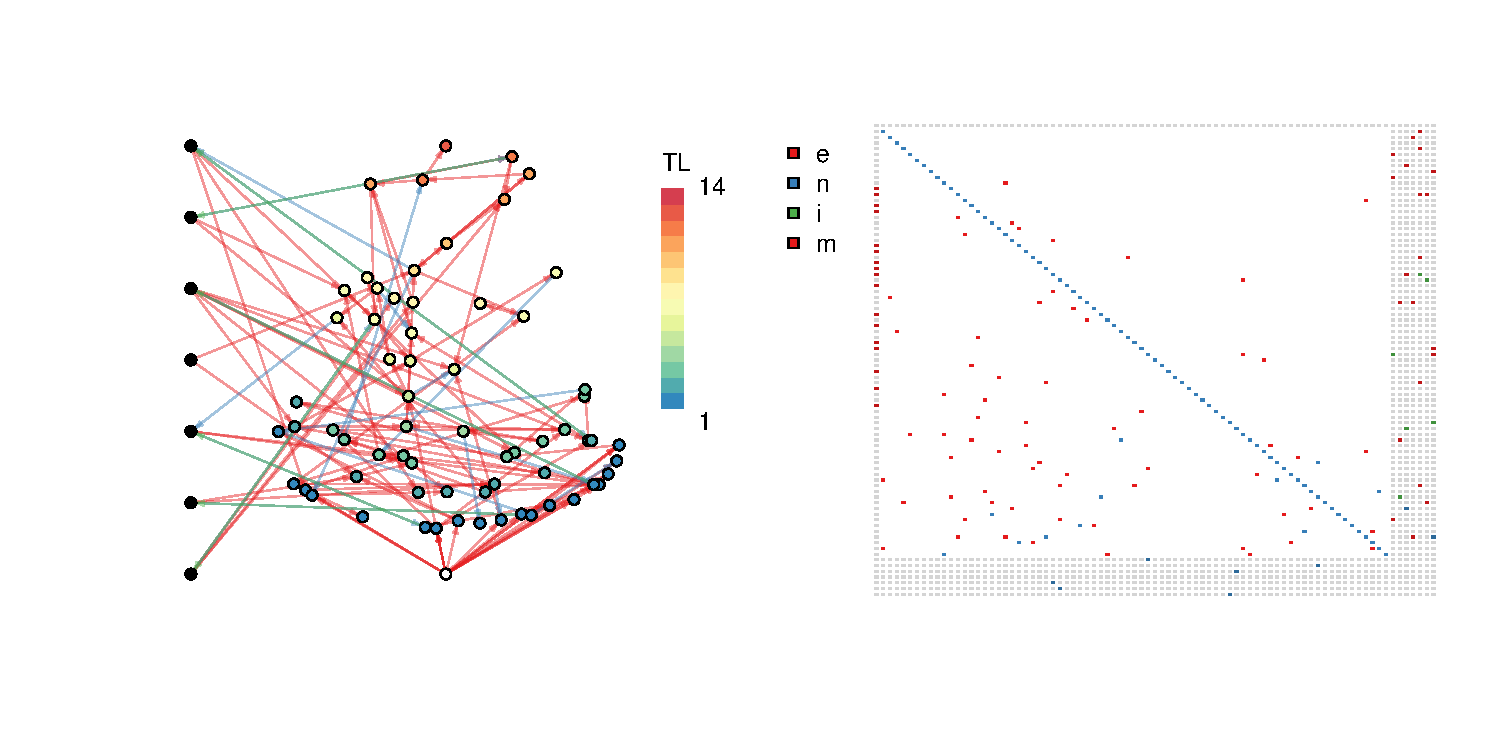
\includegraphics[width=0.5\textwidth]{fig_model.pdf}
\vspace{-6mm}
\caption{
A. Multitype interactions between species (colored nodes) and abiotic modifiers (black nodes).
B. An assembling food web with species (colored nodes; color denotes trophic level, TL) and modifiers (black nodes). The basal resource is the white node rooted at the bottom of the network.
C. The corresponding adjacency matrix with colors denoting interactions between biotic (species) and abiotic (modifiers) entities.
D. A species ($\ast$) can colonize a community when a single trophic and all service requirements are met.
E. Greater vulnerability increases the risk of primary extinction via competitive exclusion (competition denoted by dashed line) to species ($\dag$).
The extinction of species ($\dag$) will cascade to affect those connected by trophic ($\dag \dag$) and service ($\dag \dag \dag$) dependencies. 
\vspace{-3mm}
}
\vspace{-3mm}
\label{fig:model}
\end{figure}

% 1) connectance
Assembly of ecological communities in the absence of engineering results in interaction networks with structures consistent with empirical observations.
As the community reaches steady state, we find that the connectance of trophic interactions ($C=L/S^2$, where $S$ is species richness and $L$ is the number of links) decays to a value similar to that of the source pool (Fig. \ref{fig:conn}).
% The species richness of the community increases to $S_{\bm A}=130$.
Decaying connectance has been documented in the assembly of mangrove communities \cite{Piechnik2008}, however this decay is a statistical inevitability, as early in the assembly process small food webs will have high link density, from which it can only decline.
% That the connectance of assembled communities is greater than the source pool is due to the fact that only species connected by trophic interactions can enter the community to begin with, increasing expected link density compared to the overall pool.
Compared to trophic networks constructed using the Niche model \cite{Williams2000} given similar species richness and connectance, our framework results in networks with degree distributions of similar means but with reduced variance (Supporting Information, section II).

% 
% \begin{figure}
% \centering
% 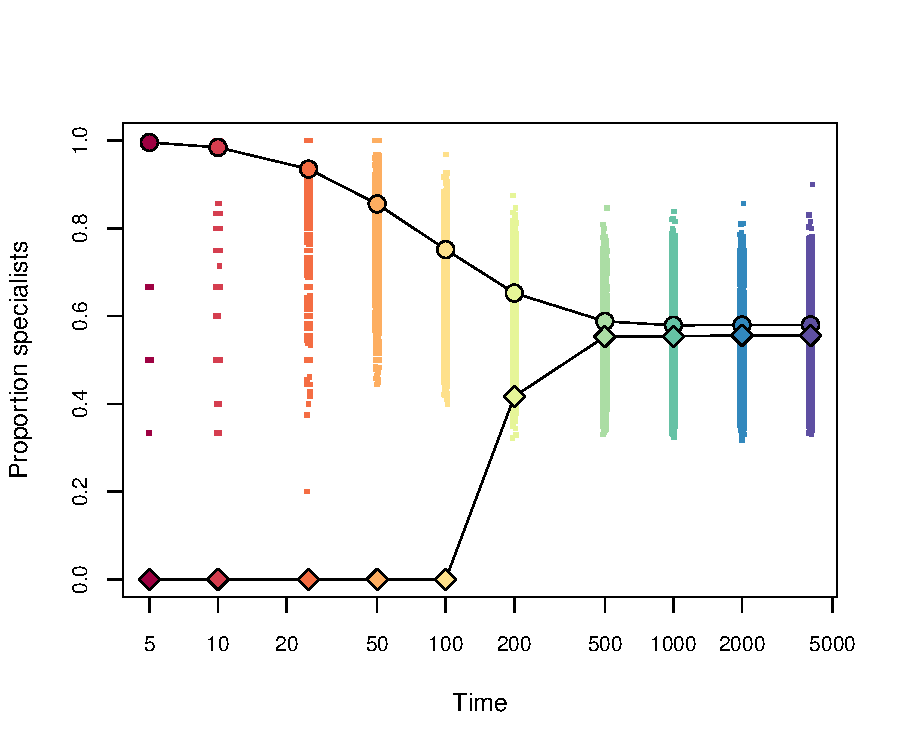
\includegraphics[width=0.5\textwidth]{fig_specialization.pdf}
% \caption{
% The proportion of specialists as a function of assembly time, where a specialist is defined as a species with a generality index $G_i < 1$.
% All measures of $G_i$ are scaled by the average number of links per species $L/S$, and we consider different values of $L/S$ on $G_i$:
% Circles: $G_i^{\rr{all}}$ where $L$ accounts for all links in the food web and $S$ accounts for all species relative to each time interval in the assembly process (averaged across replicates);
% Points: $G_i^{\rr{hetero}}$, where we consider only the links and species richness of heterotrophs, excluding autotrophs (each point shows an individual replicate);
% Diamonds: $G_i^*$, where $L$ and $S$ are measured with respect to the communities at steady state, which is most similar to the measure used to evaluate assembling mangrove food webs (averaged across replicates).
% }
% \label{fig:spec}
% \end{figure}




%Generality
Recent empirical work has suggested that generalist species may predominate early in assembly, whereas specialists colonize after a diverse resource base has accumulated \cite{Piechnik2008,Gravel2011}.
Here the trophic generality of species $i$ is defined $G_i = k^{\rm in}_i/(L/S)$ where $k^{\rm in}_i$ is the in-degree, or number of resources consumed, by species $i$ \cite{Williams2000}.
A species is classified as a generalist if $G_i > 1$ and a specialist if $G_i < 1$.
If generalism is scaled to the steady state link density (see Supporting Information, section III), we observe that generalists dominate early in assembly, with an increase in specialists as assembly progresses (Fig. \ref{fig:trophic}B).
This confirms expectations from the trophic theory of island biogeography \cite{Gravel2011}, where early communities with lower richness are less likely to support specialist consumers than late, species-rich communities.
% where communities with lower richness (early in assembly) are more likely to support generalist consumers than communities with higher richness (late in assembly). 
At steady state the proportion of specialists is ca. 56\%, similar to empirical observations of assembling food webs \cite{Piechnik2008}.
%, all measures of $L/S$ are approximately equivalent, and


%trophic levels
%Trophic Levels & degree dists
The role of specialists early in assembly is primarily due to the accumulation of autotrophic specialists.
This is evident when we observe that the trophic level (TL) distribution early in assembly ($t=5$) has an average ${\rm TL}=1.6$.
% Additional consumers arrive in the form of both mixotrophs (consuming the basal resource and one or more autotrophs) and heterotrophs, which establish higher trophic levels.
Four trophic levels are typically established by $t=50$, where colonization is still dominant, and by the time communities reach steady state the interaction networks are characterized by an average ${\rm TL_{max}}$ ($\pm$ standard deviation) $=11 \pm 2.8$ (Fig. \ref{fig:trophic}C).
While the maximum trophic level is higher than that measured in most predator-prey systems \cite{Williams2002}, it is not unreasonable if parasitic interactions (which we do not differentiate from other consumers) are included \cite{Lafferty2006}.
Overall, the most common trophic level among species at steady state is ca. ${\rm TL}=4.75$. %, which is similar to average measures  \cite{Williams2002}.

The distribution of trophic levels changes shape over the course of assembly.
Early in assembly, we observe a skewed pyramidal structure, where most species feed from the base of the food web.
At steady state, we observe that intermediate trophic levels dominate, with frequencies taking on an hourglass structure (purple bars, Fig. \ref{fig:trophic}C).
Compellingly, the trophic richness pyramids that we observe at steady state follow closely the hourglass distribution observed for empirical food webs and are less top-heavy than those produced by static food web models \cite{Turney2016}.\\




% We emphasize that these structures are diversity-weighted rather than biomass or abundance-weighted as is often the case \cite{Trebilco2013,Gibert2019}.
% Trophic levels higher than 7 do occur, but are rare.

%Cascading extinctions: Thebault
%Assembly patterns: Barbier
%Origin of ecological structure: Stokstad


%Drossel
% [RELATE TO TROPHIC ASSEMBLY MODELS]\\
%Hourglass food webs are predicted for systems where body size increases with trophic position (marine systems)



% 4) Increased mutualisms => greater nestedness
\vspace{-3mm}
\noindent \textbf{Structure and dynamics of mutualisms}\\
Nested interactions, where specialist interactions are subsets of generalist interactions, are a distinguishing feature of mutualistic networks \cite{Bascompte2003}.
A nested structure has been shown to maximize the structural stability of mutualistic networks \cite{Rohr2014}, emerge naturally via adaptive foraging behaviors \cite{Valdovinos2016,Valdovinos2019} and neutral processes \cite{Krishna2008}, and promote the influence of indirect effects in driving coevolutionary dynamics \cite{Guimaraes2017}.
While models and experiments of trophic networks suggest that compartmentalization confers greater stabilizing properties \cite{Stouffer2011,Gilarranz2017}, interaction asymmetry among species may promote nestedness in both trophic \cite{Araujo2010} and mutualistic systems \cite{Pires2011}.
Processes that operate on different temporal and spatial scales may have a significant influence on these observations \cite{Massol2011}.
For example, over evolutionary time, coevolution and speciation may degrade nested structures in favor of modularity \cite{Ponisio2019}, and there is some evidence from Pleistocene food webs that geographic insularity may reinforce this process \cite{Yeakel2013}.

\vspace{-4mm}
\begin{figure}[h!]
\centering
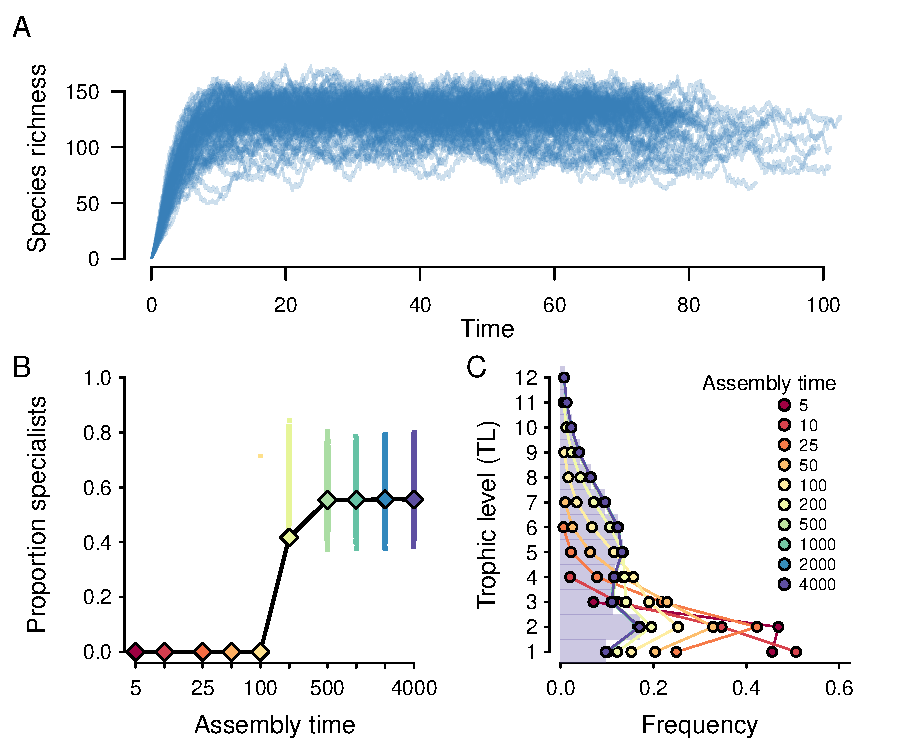
\includegraphics[width=0.5\textwidth]{fig_trophic2.pdf}
\vspace{-6mm}
\caption{
A. Assembling communities over time from a pool of 200 non-engineering species. 
Steady state species richness is reached by $t=250$.
B. The proportion of specialists as a function of assembly time (iterations), where a specialist is defined as a species with a generality index $G_i < 1$.
All measures of $G_i$ are scaled by the average number of links per species where $L$ and $S$ are measured at steady state.
C. The frequency distribution of trophic levels as a function of assembly time (iterations). 
Autotrophs occupy ${\rm TL}=1$.
Measures were evaluated across $10^4$ replicates; see Materials and Methods for parameter values.
\vspace{-3mm}
}
\label{fig:trophic}
\end{figure}


Does the assembly of ecological networks favor nestedness when mutualistic interactions are frequent?
Increasing service dependencies (\emph{need} interactions; see Fig. \ref{fig:model}) promotes both service-resource and service-service dependencies.
Consider how species with more service interactions compare to those with fewer.
More service interactions \emph{i}) increase a species' competition strength, lowering its primary extinction risk while also \emph{ii}) increasing inter-species dependencies and its secondary extinction risk.
% As such, elimination of a species that provides a service will result in the secondary extinction of the species that receives that service.
While mutualisms convey fitness advantages in order to evolve, the latter highlights the potential risk associated with losing mutualistic partners \cite{Bond1994,Colwell2012}.
Indeed, the balance that mutualists must maintain with their partners may have large implications for the future of global biodiversity \cite{Dunn2009}.



We find that as we increase the frequency of mutualistic interactions, the assembled community at steady state becomes more nested (Fig. \ref{fig:nest}).
% That the absolute values of nestedness are low compared to those measured for empirical mutualistic networks is unsurprising: observations of mutualistic interactions are generally for bipartite networks and isolated to specific systems (e.g. ant-plant mutualisms).
% Here the NODF metric is taken across both eat and need interactions across the entire assembled community.
In this case, nestedness emerges from the assembly process and provides structural robustness.
The robustness can be observed by examining the exclusionary differences between species in a simple nested motif (Fig. \ref{fig:nest}, inset).
In the trophic motif, species with high vulnerability (multiple predators) are at greater risk of primary extinction via competitive exclusion.
This will result in the secondary extinction of the specialist consumer, rendering the nested structure prone to change.
In our framework mutualistic networks are generally formed by composite interactions, where the consumer species is engaged in a trophic interaction while the resource species is engaged in a service interaction.
As such, the consumer species becomes a trophic partner and the resource species gains the competitive advantages of the service.
If the competitive advantages of services are greater than the costs of vulnerability (see Materials and Methods), it is the low vulnerability species with fewer trophic partners that is at greater risk of exclusion (Fig. \ref{fig:nest}, inset).
Because its elimination will not cascade, the nested structure will be more resistant to change.


Our results also suggest that the addition of mutualistic interactions comes at a cost to the assembling community.
Because mutualisms increase dependencies between species, they also increase the frequency of secondary extinctions (Fig. \ref{fig:nest}).
% , we observe that these networks have lower species' persistence
 %as well as lower diversity (Supplemental Materials).
% both lower species diversity on average as well as lower species' persistence.
Measuring persistence in terms of the proportion of time species are established in the network reveals that more frequent mutualisms leads on average to lower persistence.
% Persistence as measured as the percent simulation time the community is occupied by a given species, averaged across all species that successfully colonize.
At the community-scale, lower average persistence implies greater species turnover.
Observations of empirical systems appear to support our model predictions.
For example, assembling plant-pollinator systems have demonstrated high rates of species and interaction turnover, both during the assembly process and at the steady state \cite{Ponisio2017}.
% Ponisio et al. \cite{Ponisio2017} suggested that the assembly process they observed was ordered by an `opportunistic attachment' rather than `preferential attachment' process, where generalist interactions reordered in response to the changing conditions of the community.
% The framework that we present here employs an attachment dynamic that is more in line with an opportunistic, rather than preferential, process, as invoked by Ponisio et al. \cite{Ponisio2017} to explain observed changes in mutualism structure over the course of assembly.
% Our results suggest that such a process, when employed in randomly assembled multitype interaction networks, results in THE STRUCTURE AND DYNAMICS EXPECTED OF ASSEMBLING MUTUALISTIC SYSTEMS.


\begin{figure}[h!]
\centering
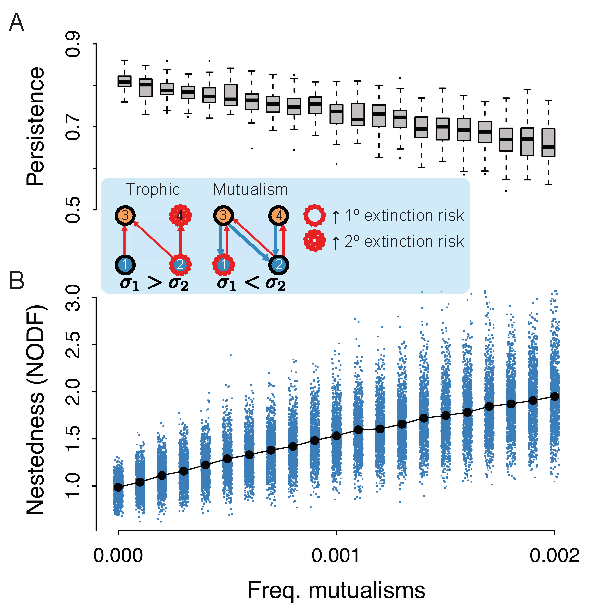
\includegraphics[width=0.5\textwidth]{fig_nested2.pdf}
\vspace{-8mm}
\caption{
A. Species persistence with increasing frequencies of mutualistic (service) interactions without ecosystem engineers.
% Persistence as measured as the percent simulation time the community is occupied by a given species, averaged across all species that successfully colonize.
B. Structural nestedness of communities, measured as NODF (Nestedness based on Overlap and Decreasing Fill) \cite{AlmeidaNeto2008}.
Measures were evaluated across $10^4$ replicates; see Materials and Methods for parameter values.
Inset: A trophic and mutualistic nested motif for resource species 1, 2 and consumer species 3, 4.
Trophic motif: the vulnerable species 2 is subject to primary extinction because it has a lower competition strength $\sigma$, resulting in an extinction cascade of species 4.
Mutualistic motif: the least vulnerable species 1 with fewer mutualistic partners is subject to primary extinction without cascading effects.
\vspace{-6mm}
}
\label{fig:nest}
\end{figure}


% An important condition of our model is that we assume that all service interactions are obligate (see Materials and Methods), which is expected to heighten the influence of secondary extinctions.
We emphasize that we have restricted ourselves to examining the effects of obligate mutualisms, although the importance of non-obligate mutualisms has long been recognized \cite{Ramos2012,Vieira2015,Valdovinos2016,Ponisio2017,Valdovinos2019}.
% Because including these
While the inclusion of non-obligate mutualists will lower the likelihood of cascading effects in systems with higher frequencies of service interactions, the loss of obligate mutualistic partners will have larger dynamic consequences than the loss of more flexible non-obligate mutualistic partners.
As such, we do not expect inclusion of non-obligate mutualisms to alter the qualitative nature of our findings.\\
% In future efforts, we aim to explore how the combination of obligate and non-obligate mutualisms impact community dynamics.
% In future efforts, we aim to explore the effects of both obligate and non-obligate mutualistic interactions on community assembly.\\
%What is the CV of mutualistic trajectories?




\vspace{-3mm}
\noindent \textbf{Assembly with ecosystem engineering}\\
%Theory
The concept of ecosystem engineering, or more generally niche construction, has both encouraged an extended evolutionary synthesis \cite{Laland2015} while also garnering considerable controversy \cite{Gupta2017,Feldman2017}.
Models that explore the effects of ecosystem engineering are relatively few, but have covered important ground \cite{Hastings2007,OdlingSmee2013}.
For example, engineering has been shown to promote invasion \cite{Cuddington2004}, alter primary productivity \cite{Wright2004}, and change the selective environment over eco-evolutionary timescales \cite{Kylafis2008,Krakauer2009} which can lead to unexpected outcomes such as the fixation of deleterious alleles \cite{Laland1999}.
% Initial work focused on understanding how habitat modification might impact the persistence of engineering species \cite{Gurney1996}, while more recent efforts have shown that engineering can promote invasion \cite{Cuddington2004} and impact primary productivity \cite{Wright2004}.
% On eco-evolutionary timescales, ecosystem engineering can alter the selective environment \cite{Krakauer2009,OdlingSmee2013} and ultimately lead to unexpected outcomes such as the fixation of deleterious alleles \cite{Laland1999}.
% On macroevolutionary timescales, there is considerable interest in understanding the role of innovation on diversification and extinction rates within and among clades \cite{Marshall2016}.
% While such innovation generally pertains to the appearance of morphological traits, environmental modifications that result from evolutionary innovations can sometimes be wide-ranging, such as the planetary-scale consequences following the evolution of multicellular cyanobacteria \cite{Schirrmeister2013}.
On smaller scales, microbiota construct shared metabolitic resources that have a significant influence on microbial communities \cite{Kallus2017}, the dynamics of which may even serve as the missing ingredient stabilizing some complex ecological systems \cite{Muscarella2017}.


We next explore the effects of ecosystem engineering by allowing species to produce abiotic modifiers as additional nodes in the ecological network (Fig. \ref{fig:model}).
These modifier nodes produced by engineers can serve to fulfill resource or service requirements for other species.
The parameter $\eta$ defines the mean number of modifiers produced per species, drawn from a Poisson distribution (see Materials and Methods for details).
Increasing the frequency of engineering interactions both increases the number of engineering species (those species making $\geq 1$ modifier) and the number of modifiers per species.
There are two characteristics of engineering that have particular relevance for community assembly:
modifiers can linger in the community even after the species that produce them have been excluded, and
more than one engineer can produce the same modifier such that engineering redundancies increase with $\eta$ (Supporting Information, section I).




%Engineering can produce positive feedback dynamics on engineers
%Positive feedback over evolutionary time => speciation/radiation
%Lead to engineering redundancies
%This may be rare as Lawton suggests, but appears to be quite common in the microbial world.
%In microbiomes, horizontal gene transfer can produce redundant engineering without radiations

%Lawton 1994: there may be sometimes redundancy in ecosystem engineers... (uses beaver to suggest that there is not)

%negative (introduces dependencies) then positive (introduces redundancies)
Increasing engineering has significant consequences for community robustness, but these effects also are sensitive to the frequency of service interactions within the community.
We measure community robustness by 
\emph{i}) rates of primary versus secondary extinctions,
\emph{ii}) species persistence, and 
\emph{iii}) steady state community diversity.
% Primary extinctions result from the competitive exclusion of species, whereas secondary extinctions are those that occur as a direct result of the former.
All measures were averaged over each species within the community across assembly time.

% Increasing engineering has different effects on primary versus secondary extinctions.
As the number of engineers increase, mean rates of primary extinction are first elevated and then decline (Fig. \ref{fig:engineers}A).
This nonlinear effect of engineering on rates of primary extinction results from two competing forces.
Increased production of abiotic modifiers supplies consumers with additional resources, limiting secondary extinctions and promoting persistence (Fig. \ref{fig:engineers}B,~C).
However, the stabilization of consumers ultimately results in increased vulnerability of prey.
 % while also increasing the vulnerability of prey.
Engineering dependencies are considered rare when the ratio of modifier nodes per species is $0 < \eta \leq 0.5$.
The cumulative effect in these species-rich/modifier-poor systems is increased competitive exclusion of prey and higher rates of primary extinction (Fig. \ref{fig:engineers}A).
Notably the presence of even a small number of engineers serves to limit the magnitude of secondary extinction cascades.
% In contrast, rates of secondary extinction decline and species' persistence increase as engineering creates abundant niche space (Fig. \ref{fig:engineers}B).
% Lower species' persistence => species' turnover.
Higher rates of primary extinction coupled with lower rates of secondary extinction mean that extinctions are common, but of limited magnitude such that disturbances are compartmentalized.
As engineering becomes common ($\eta > 0.5$) the available niche space expands, lowering competitive overlap and suppressing both primary and secondary extinctions.
% ecological networks are least stable when engineers are rare, and most stable when engineers are common.

%Mutualisms + Engineering
Increasing the frequency of service interactions promotes service interactions between species and engineered modifiers (Fig. \ref{fig:model}).
A topical example of the latter is the habitat provided to invertebrates by the recently discovered rock-boring teredinid shipworm (\emph{Lithoredo abatanica}) \cite{Shipway2019}.
Here, freshwater invertebrates are serviced by the habitat modifications engineered by the shipworm, linking species indirectly via an abiotic effect (in our framework via a modifier node).
As the frequency of service interactions increases, the negative effects associated with rare engineers is diminished (Fig. \ref{fig:engineers}A).
Increasing service interactions both elevates the competitive strength of species receiving services (from species and/or modifiers), while creating more interdependencies between and among species.
% Species that serve as resources to many consumers are less competitive due to increased vulnerability.
As trophic interactions are replaced by service interactions, previously vulnerable species gain a competitive foothold and persist (Fig. \ref{fig:nest}, inset), lowering rates of primary extinctions (Fig. \ref{fig:engineers}A). %, particularly in systems where consumers are facilitated by a small number of engineers
The costs of these added services to the community are an increased rate of secondary extinctions (Fig. \ref{fig:engineers}B) and higher species turnover (Fig. \ref{fig:engineers}C).
Low rates of primary extinction coupled with high rates of secondary extinction mean that extinctions are less common but lead to larger cascades.
% Importantly, these changes are not due to fluctuations in steady state community richness, which remains relatively constant across the parameter space that we examine (Fig. \ref{fig:steadystate}A).

% Together, these results point to an important tradeoff originating from the effects of engineering.
% When engineering and servive interactions are rare, extinction rates are higher, but have smaller consequences; as mutualisms become more common, extinction rates are lower, but have larger consequences.


% Ecosystem engineers can be stabilizing agents in communities if they primarily serve to provide additional resources to non-specialist consumers.
% However if species' presence in the community require the effects induced by engineers, their cumulative influence can be destabilizing.
% Whether engineers are stabilizing or destabilizing is thus largely determined by the flexibility of inter-dependencies connecting species in a community.
% Redundancy in engineered effects both lowers extinction rates while increasing the time that individual species are present within the assembling community.

\vspace{-4mm}
\begin{figure}[h!]
\centering
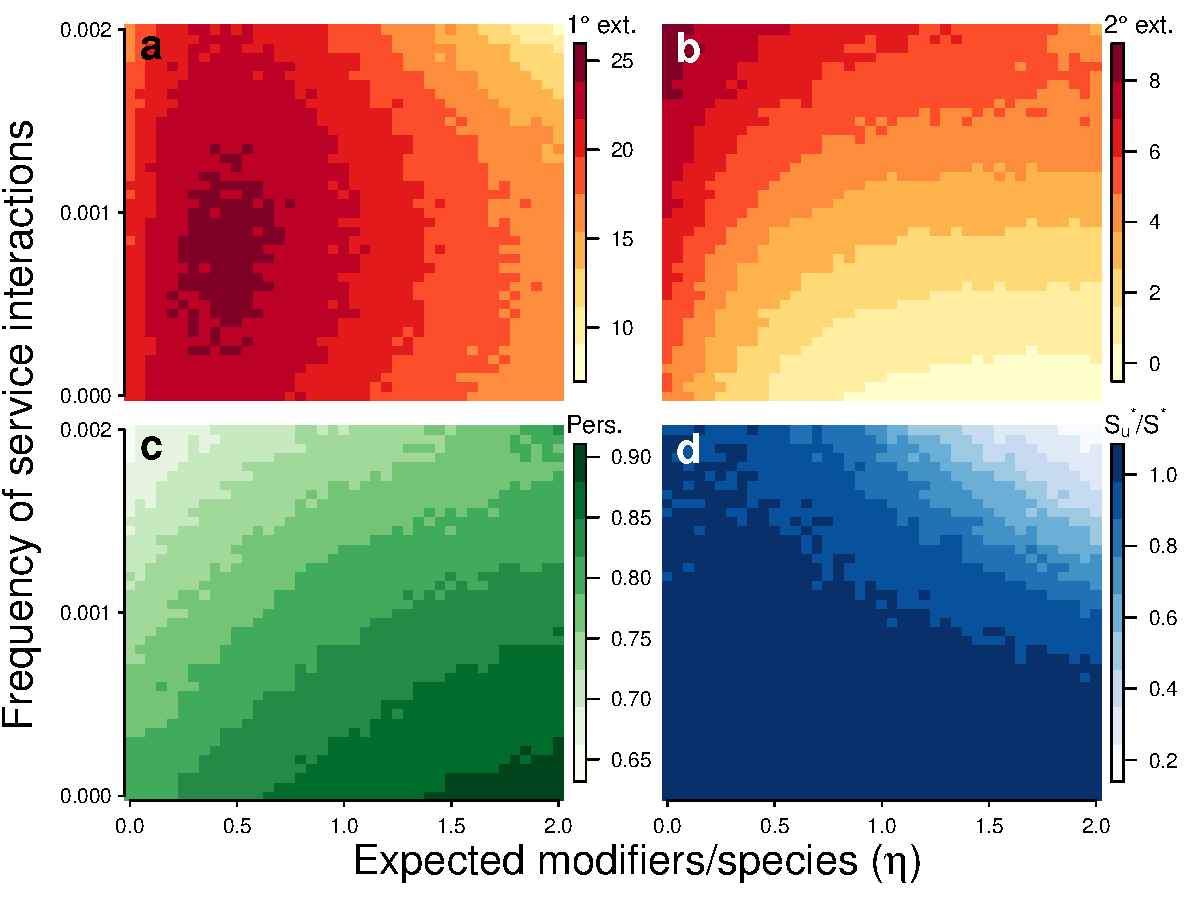
\includegraphics[width=0.5\textwidth]{fig_engineers4.pdf}
\vspace{-8mm}
\caption{
Community robustness as a function of the frequency of service interactions and modifiers per species.
A. Mean rates of primary extinction, where primary extinctions occur from competitive exclusion of consumers over shared resources.
B. Mean rates of secondary extinction, which cascade from primary extinctions.
C. Mean species persistence.
D. The ratio $S^*_{\rm u}/S^*$, where $S^*_{\rm u}$ denotes steady states for systems where all engineered modifiers are unique to each engineer, and $S^*$ denote steady states for systems with redundant engineering. Lower values of $S^*_{\rm u}/S^*$ mean that systems with redundant engineers have higher richness at the steady state than those without redundancies.
Measures were evaluated across $50$ replicates; see Materials and Methods for parameter values.
\vspace{-5mm}
}
\label{fig:engineers}
\end{figure}



While the importance of engineering timescales has been emphasized previously \cite{Hastings2007}, redundant engineering has been assumed to be unimportant \cite{Lawton1994}.
We argue that redundancy may be an important component of highly engineered systems, and particularly relevant when there exists a positive feedback between the effects of engineers on their fitness \cite{Cuddington2004}.
The vast majority of contemporary ecosystem engineering case studies focus on single taxa, such that redundant engineers appear rare \cite{Lawton1994}.
However if we consider longer timescales, increasing diversity of engineering clades may promote redundancy, and in some cases this may feed back to accelerate diversification \cite{OdlingSmee2013b}.
Such positive feedback mechanisms likely facilitated the global changes induced by cyanobacteria in the Proterozoic \cite{Erwin2008,Schirrmeister2013} among other large-scale engineering events in the history of life \cite{Erwin2008}.
Engineering redundancies are likely important on shorter timescales as well.
For example, diverse sessile epifauna on shelled gravels in shallow marine environments are facilitated by the engineering of their ancestors, such that the engineered effects of the clade determine the future fitness of descendants \cite{Kidwell1986}.
In the microbiome, redundant engineering may be very common due to the influence of horizontal gene transfer in structuring metabolite production \cite{Polz2013}.
In these systems, redundancy in the production of shared metabolitic resources may play a key role in community structure and dynamics \cite{Kallus2017,Muscarella2017}.




% %Role of Redundancy
When there are few engineers, each modifier in the community tends to be unique to a particular engineering species.
Engineering redundancies increase linearly with $\eta$ (Supporting Information, section I; Fig. \ref{fig:redundancy}), such that the loss of an engineer will not necessarily lead to the loss of engineered modifiers. % if alternative engineers persist.
We examine the effects of this redundancy by comparing our results to those produced by the same model, but where each modifier is uniquely produced by a single species.
Surprisingly, the lack of engineering redundancies does not alter the general relationship between engineering and measures of community robustness (Fig. \ref{fig:unique}).
However we find that redundancies play a central role in maintaining species diversity.
When engineering redundancies are allowed, steady state community richness $S^*$ does not vary considerably with increasing service interactions and engineering (Fig. \ref{fig:steadystate}A).
In contrast, when redundant engineering is not allowed, steady state community richness $S^*_u$ declines sharply (Figs. \ref{fig:engineers}D, \ref{fig:steadystate}B).

Communities lacking redundancy have lower species richness because sparse interdependencies preclude colonization (Fig. \ref{fig:steadystate}C,D).
Colonization occurs only when trophic and service dependencies are fulfilled.
A species requiring multiple engineered modifiers, each uniquely produced, means that each required entity must precede colonization.
This magnifies the role of priority effects in constraining assembly order \cite{Fukami2015}, precluding many species from colonizing.
In contrast, redundancy increases the niche space available to species while minimizing priority effects by allowing multiple engineers to fulfill dependencies.
Our results thus suggest that redundant engineers may play important roles in assembling ecosystems by lowering the barriers to colonization thereby promoting community diversity.



% When service interactions are common, the presence of a few engineers reduces stability because there are more dependencies between species and modifiers that must be maintained.
% However if engineering continues to increase, greater dependencies are offset by increased redundancy.
% If engineers and the modifiers they create are redundant, service interactions can be maintained even when engineers go extinct.
% In contrast, species persistence is not strongly penalized by the lack of engineering redundancy \ref{fig:engineers}B), however we observe that the beneficial effects of engineering is reduced.
% 
% 
% %Without mutualists: engineering always GOOD
% When service interactions are absent, we find that increasing engineering both lowers extinction rates and increases species persistence (Fig. \ref{fig:engineers}).
% 
% Moreover, when most species are engineers ($\eta = 2$), the probability that a single modifier has two or more engineers is high.
% This added redundancy means that the disappearance of a single engineer has a lower impact on the community, further promoting stability.



% 
% In our framework, service interactions are less flexible than trophic interactions: while just a single trophic interaction is required to avoid extinction, all service interactions must be realized.
% In systems with higher frequencies of service interactions, extinction rates first increase with engineering and then decline (Fig \ref{fig:engineers}A).
% In contrast, species persistence increases with engineering but at a slower rate compared to systems without service interactions (Fig \ref{fig:engineers}B).
% 
% 
% Because modifiers linger in the community following the extinction of an engineer, their presence diffuses the risks of cascading effects originating from competitive exclusion.
% 

%Closing
Together, the results of our model point to the importance of considering multitype interactions both between species and as mediated through changes to the environment via engineering.
We suggest that including the effects of engineers, either explicitly as we have done here, or otherwise, is vital for understanding the inter-dependencies that define ecological systems.
As past ecosystems have fundamentally altered the landscape on which contemporary communities interact, future ecosystems will be defined by the influence of engineering today.
Understanding the role of ecosystem engineers is thus tantamount to understanding our own.\\


% \noindent \textbf{Beyond engineering}
%NOTE: THIS IS DISCUSSION MATERIAL

%EVOLUTION: CITE LOEUILLE, Fussmann, Allhoff 2013,2015; Brannstrom








% \begin{matmethods}
\vspace{-2mm}
\noindent \textbf{Materials and Methods}\\
  \footnotesize{
  % \noindent \textbf{The ENIgMa Model}\\
  We model an ecological system with a network where nodes represent \emph{ecological entities} such as populations of species and or the presence of abiotic modifiers affecting species such as (examples).
   % and links represent interactions between them.
  Following Pilai et al. \cite{Pillai2011}, we do not track the abundances of entities but only track their presence or absence.
  The links of the network represent interactions between pairs of entities (x,y).
  We distinguish three types of such interactions: x eats y, x needs y to be present, x makes modifier y.

  The assembly process entails two steps: first a source pool of species is created, followed by colonization/extinction into/from a local community.
  The model is initialized by creating $S$ species and $M = \eta S$ modifiers, such that $N=S+M$ is the average total number of entities and $\eta$ is the average number of modifiers per species in the system.
  For each pair of species (x,y) there is a probability $p_e$ that x eats y and probability $p_n$ that x needs y.
  For each pair of species x and modifier m, there is a probability $q_e$ that x eats m and a probability $q_n$ that species x needs modifier m.
  Additionally, each species makes a number of modifiers that is drawn from a Poisson distribution with mean $\mu = \eta e/(e-1)$ where $e$ is Euler's number.
  Once the number of modifiers per species is determined, each modifier is assigned to a species independently.
  This means that multiple species may make the same modifier, and that there may be some modifiers that are not made by any species, which are eliminated from the pool.

  In addition to interactions with ecosystem entities, there can be interactions with a basal resource, which is always present.
  The first species always eats this resource, such that there is always a primary producer in the pool.
  Other species eat the basal resource with probability $p_e$.
  Species with zero assigned trophic interactions are assumed to be primary producers.
  See Supporting Information, section I for additional details on defining the source pool.

  We then consider the assembly of a community which at any time will contain a subset of entities in the pool and always the basal resource.
  In time, the entities in the community are updated following a set of rules.
  A species from the pool can colonize the community if the following conditions are met:
  1) all entities that a species needs are present in the community, and
  2) at least one entity that a species eats is present in the community.
  If a colonization event is possible, it occurs stochastically in time with rate $r_\rr{c}$.

  An established species is at risk of extinction if it is not the strongest competitor at least one of its resources that it eats.
  We compute the competitive strength of species $i$ as
  \begin{equation}
    \sigma_i = c_\rr{n} n_i - c_\rr{e} e_i - c_\rr{v} v_i,
  \end{equation}
  where $n_i$ is the number of entities that species $i$ needs, $e_i$ is the number of entities from the pool that species $i$ can eat, and $v_i$ is the number of species in the community that eat species $i$.
  This captures the ecological intuition that mutualisms provide a fitness benefit, specialists are stronger competitors than generalists, and many predators entail an energetic cost.
  The coefficients $c_\rr{n},~c_\rr{e},~c_\rr{v}$ describe the relative effects of these contributions to competitive strength.
  In the following, we use the values $c_\rr{n} > c_\rr{e} > c_\rr{v}$, such that the competitive benefit of adding an additional mutualism is greater than the detriment incurred by adding another prey or predator.
  % In the following, we use the values $c_\rr{n} = \pi,~c_\rr{e}=\sqrt{2},~c_\rr{v}=1$, such that the competitive benefit of adding an additional mutualism is greater than the detriment incurred by adding another prey or predator.
  A species at risk of extinction leaves the community stochastically in time at rate $r_e$.

  A modifier is present in the community whenever at least one species that makes the modifier is present.
  If a species that makes a modifier colonizes a community, the modifier is created immediately, however modifiers may persist for some time after the last species that makes the modifier goes extinct.
  Any modifier that has lost all of its makers disappears stochastically in time at rate $r_m$.

  The model described here can be simulated efficiently with an event-driven simulation utilizing a Gillespie algorithm.
  In these types of simulations, one computes the rates $r_j$ of all possible events $j$ in a given step.
  One then selects the time at which the next event happens by drawing a random number from an exponential distribution with mean $1/\sum_j{r_j}$.
  At this time, an event occurs that is randomly selected from the set of possible events such that the probability of event $a$ is $r_a/\sum_j{r_j}$.
  The effect of the event is then realized and the list of possible events is updated for the next step.
  This algorithm is known to offer a much better approximation to the true stochastic continuous time process than a simulation in discrete time steps, while providing a much higher numerical efficiency \cite{Gillespie1977}.
  Simulations described in the main text have default parameterizations of $S=200$, $p_{\rm e}=0.01$, $c_{\rm n} = \pi$, $c_{\rm e} = \sqrt{2}$, $c_{\rm v} = 1$, and $4000$ iterations.}
% \end{matmethods}

% 
% 
% \begin{table*}[!t]
% \begin{center}
% \begin{tabular}{ l l l }
% \hline
% Parameter & Definition & Value/Range \\
% \hline
% $\overrightarrow{a}$ & assimilate & \\
% $\overrightarrow{n}$ & need & \\
% $\overrightarrow{i}$ & ignore & \\
% $\overrightarrow{m}$ & make & \\
% \hline
% $e \leftrightarrow i$ & Asymmetric consumption & $p_{ei} = p_i(p_e/(p_e+p_n+p_i)) + p_e(p_i/(p_a+p_i+p_n))$ \\
% $e \leftrightarrow e$ & Symmetric consumption & $p_{ee} = p_e(p_e/(p_i+p_n+p_e))$\\
% $e \leftrightarrow n$ & Trophic mutualism & $p_{en} = p_n(p_e/(p_e+p_n+p_i+p_m)) + p_e(p_n/(p_a+p_i+p_n))$ \\
% $n \leftrightarrow n$ & Non-trophic mutualism & $p_{nn} = p_n(p_n/(p_e+p_n+p_i+p_m))$ \\
% $n \leftrightarrow i$ & Commensalism & $p_{ni} = p_n(p_i/(p_e+p_n+p_i+p_m)) + p_i(p_n/(p_e+p_n+p_i))$\\
% $m \leftrightarrow n$ & Engineering & $p_{mn} = p_n(p_m/(p_e+p_n+p_i+p_m)) + p_m$\\
% $i \leftrightarrow i$ & Null & $p_{ii} = p_i(p_i/(p_e+p_n+p_i))$\\
% \hline
% $\mathcal{N}$ & Number of species + modifiers & dyn.\\
% $\mathcal{S}$ & Number of species & dyn.\\
% $\mathcal{M}$ & Number of modifiers & dyn.\\
% \hline
% \end{tabular}
% \end{center}
% \caption{Table of parameters, definitions, and assigned values or ranges.}
% \label{table:param}
% \end{table*}
% 



%
% \textbf{Building the source pool} The source pool interaction matrix $\bm P$ is generated by first setting the number of species in the pool $\mathcal{S}_{\bm P}$ and determining the number of modifiers $\mathcal{M}_{\bm P}$ that are made by ecosystem engineers.
% The resulting matrix is $\mathcal{N}_{\bm P}\times\mathcal{N}_{\bm P}$ where $\mathcal{N}_{\bm P}=\mathcal{S}_{\bm P}+\mathcal{M}_{\bm P}$, and is subdivided into four quadrants, only two of which play a role here: species-species interactions and species-modifier interactions (see Fig. \ref{fig:matrix}).
% In these two quadrants, the expected frequency of eat interactions ${\rm E}\{p_\rr{e}\}$ and the expected frequency of need interactions ${\rm E}\{p_\rr{n}\}$ are free parameters, as is the expected number of modifiers made per species ${\rm E}\{\mathcal{M}_i\}=\eta$.
% Here and throughout, we simplify this parameter space by assuming that the frequency of eat and need interactions for species-species (SS) interactions and species-modifier (SO) interactions scale as $\phi$, such that ${\rm E_{SS}}\{p_\rr{e}\} = \phi{\rm E_{SO}}\{p_\rr{e}\}$ and ${\rm E_{SS}}\{p_\rr{n}\} = \phi{\rm E_{SO}}\{p_\rr{n}\}$.
% % is given by the parameter ${\rm E}\{\mathcal{M}_i\}=\eta$, which determines how many modifiers will be present in the source pool.
% % The source pool interaction matrix $\bm P$ is generated by first setting the number of species $\mathcal{S}$ and the expected number of modifiers that are engineered per species ${\rm E}\{\mathcal{M}_i\}=\eta$.
% For each species, a set number of modifiers is drawn from ${\rm Poiss}(\eta)$, such that the expected proportion of species that are engineers (species that make modifiers) is $1-{e}^{-\eta}$.
% If a particular modifier is randomly and independently drawn for a given engineer from a complete list of all possible modifiers, such that multiple species -- with some probability -- can make the same modifier, the expected number of modifiers is
% \begin{equation}
% {\rm E}\{\mathcal{M}_{\bm P}\} = \mathcal{S}_{\bm P}\eta\left(1 - \frac{1}{{e}}\right),
% \end{equation}
% where $e$ is Euler's number.
% % This allows multiple species to make the same modifier.
% % If each species makes unique modifiers, the number of expected modifiers is $\mathcal{M} = \mathcal{S}\eta$, however because multiple species can make the same modifier, the realized number of modifiers will be lower.
% % % To determine whether modifiers are uniquely made or made by multiple engineers, we assign modifiers by randomly drawing independently modifier IDs from $[1:\mathcal{M}_{\rm max}]$ without replacement for each engineer; unassigned modifiers are discarded.
% % Each engineer is randomly assigned a modifier, which permits a single modifier to be made by multiple engineers, such that
% % \begin{equation}
% % {\rm E}\{\mathcal{M}\} = \mathcal{S}\eta\left(1 - \frac{1}{{\rm e}}\right).
% % \end{equation}
% % where $\rm e$ is Euler's number.
% The frequency of $m \leftrightarrow n$ interactions is then calculated as
% \begin{equation}
% {\rm E}\{p_\rr{m}\} = \frac{\eta}{\mathcal{S}_{\bm P}\left(1 + \eta - \frac{\eta}{e}\right)^2}.
% \end{equation}
% Finally the frequency of the ignore interaction is calculated as $\rr{E_{SS}}\{p_\rr{\varnothing}\} = 1 - \rr{E_{SS}}\{p_\rr{e}\} + \rr{E_{SS}}\{p_\rr{n}\}$ and  $\rr{E_{SO}}\{p_\rr{\varnothing}\} = 1 - \rr{E_{SO}}\{p_\rr{e}\} + \rr{E_{SO}}\{p_\rr{n}\}+ \rr{E_{SO}}\{p_\rr{m}\}$ for species-species and species-modifier interactions, respectively.
% Pairwise interaction probabilities between both species and modifiers are then calculated as shown in Table \ref{table:param}.
% These pairwise interactions are assigned randomly from these probabilities between species-species and species-modifiers independently in both quadrants, such that the source pool matrix has no imbued structure apart from the number of species, the number of modifiers, and the frequency of each directional interaction type.
% Each source pool is provided a \emph{basal resource} (the first row/column).
% A species with a single trophic interaction to this resource is identified as a pure autotroph (Fig. \ref{fig:matrix}), however the basal resource does not have eat, need, or make interactions itself.
%
%
%
%
% We consider a framework incorporating multiple types of directional interactions between species, which, when paired, represent specific ecological relationships including trophic interactions, service-resource and service-service mutualisms, and commensalisms.
% We also introduce two types of nodes in our depiction of ecological networks: those representing \emph{species} and those representing \emph{modifiers}.
% modifiers must be made by one or more species (here and henceforth refereed to as engineers) and represent a modification to the available niche-space that can be utilized by other species in the community.
% Such alterations are to be considered in the abstract, but in empirical systems could represent an introduced compound, metabolite, or an alteration to the habitat/environment such as, for example, a burrow.
%



%
% %Interaction types
%
% The ENIgMa model consists of four directed interactions:
% $\rr{e}$: eat, which specifies a dependency involving the exchange of biomass,
% $\rr{n}$: need, which specifies a dependency that does not involve biomass flow (e.g. a reproductive service),
% $\rr{i}$: ignore, the null interaction, and
% $\rr{m}$: make, which connects a species to a modifier that it engineers.
% `modifiers' are interactive components that can be made by $\geq 1$ species, and eaten, needed, or ignored by the others.
% The four directed interaction types describe specific dependencies that one species/modifier has on another, however it is the coupling of two opposing directed interactions that describe familiar ecological relationships (Table 1).
%
% The $\rr{e} \leftrightarrow \rr{i}$ interaction describes a typical predator-prey relationship, where species 1 eats species 2, whereas aside from serving as a resource, species 2 does not interact with (ignores) species 1.
% Of course, a prey's abundance does not \emph{ignore} the effects of predation, however our framework operates at the scale of presence/absence rather than abundance, and we assume that if both species co-occur, they have positive population densities, such that the prey's state (presence/absence) ignores the predator.
% A second type of trophic interaction is described by $\rr{e} \leftrightarrow \rr{e}$, where consumption is symmetric, which could be do to changing roles over an individual's life-history.
% The $\rr{e} \leftrightarrow \rr{n}$ and $\rr{n} \leftrightarrow \rr{n}$ interactions describe service-resource and service-service mutualisms, respectively.
% In the case of the former, one species interacts by way of a trophic interaction, whereas the other is provided a non-trophic need, such is the case in a plant-pollinator relationship.
% Unique to models of ecological networks, the $\rr{m} \leftrightarrow \rr{n}$ interaction describes ecosystem engineering, where a species makes a modifier, whereas the presence of the modifier `needs' the presence of the species that makes it.
% modifiers can be utilized by other species in the community, providing an indirect dependency that could be facilitated by multiple species (many engineers make the same modifier) and/or used by multiple species (many species eat or need the same modifier).
% As we will describe below, engineers can modify the niche space available to the community on timescales that last longer than the species themselves, which is an oft-assumed characteristic of engineering.
%
% We explore the assembly of a novel community that emerges from a species source pool, which is represented by a source pool interaction matrix where all eat, need, ignore, and make interactions are established between all species and modifiers.
% As such, a set of interactions for a particular species defines how it interacts with any other \emph{a priori}, thereby establishing its potential interaction niche space.
% The source pool is used to seed a novel community, which arises as the result of colonization and extinction rules, the details of which we describe below.
%


% \bibliography{aabib}

\begin{thebibliography}{10}

\bibitem{Paine1966}
Paine RT (1966) Food web complexity and species diversity.
\newblock {\em Am. Nat.} 100(910):65--75.

\bibitem{Dunne2002}
Dunne JA, Williams RJ, Martinez ND (2002) Food-web structure and network
  theory: the role of connectance and size.
\newblock {\em Proc Natl Acad Sci USA} 99(20):12917--12922.

\bibitem{Pascual2006}
Pascual M, Dunne J (2006) {\em Ecological Networks: Linking Structure to
  Dynamics in Food Webs}.
\newblock (Oxford University Press, Oxford, UK).

\bibitem{Bascompte2013}
Bascompte J, Jordano P (2013) {\em Mutualistic Networks}, Monographs in
  Population Biology.
\newblock (Princeton University Press, Princeton, NJ).

\bibitem{May1972}
May RM (1972) {Will a large complex system be stable?}
\newblock {\em Nature} 238(5364):413--414.

\bibitem{Gross2009}
Gross T, Levin SA, Dieckmann U (2009) Generalized models reveal stabilizing
  factors in food webs.
\newblock {\em Science} 325(5941):747--750.

\bibitem{Allesina2012}
Allesina S, Tang S (2012) {Stability criteria for complex ecosystems}.
\newblock {\em Nature} 483(7388):205--208.

\bibitem{Ponisio2017}
Ponisio LC, Gaiarsa MP, Kremen C (2017) Opportunistic attachment assembles
  plant–pollinator networks.
\newblock {\em Ecol Lett} 20(10):1261--1272.

\bibitem{Guimaraes2017}
Guimar{\~a}es~Jr PR, Pires MM, Jordano P, Bascompte J, Thompson JN (2017)
  {Indirect effects drive coevolution in mutualistic networks}.
\newblock {\em Nature} 18:586.

\bibitem{Kefi2016}
K{\'e}fi S, Miele V, Wieters EA, Navarrete SA, Berlow EL (2016) How structured
  is the entangled bank? the surprisingly simple organization of multiplex
  ecological networks leads to increased persistence and resilience.
\newblock {\em PLoS Biol} 14(8):e1002527.

\bibitem{Pilosof2017}
Pilosof S, Porter MA, Pascual M, K{\'e}fi S (2017) The multilayer nature of
  ecological networks.
\newblock {\em Nature Ecol Evol} 1:0101.

\bibitem{Lawton1994}
Lawton JH (1994) What do species do in ecosystems?
\newblock {\em Oikos} 71(3):367--374.

\bibitem{OdlingSmee2013}
Odling-Smee J, Erwin DH, Palkovacs EP, Feldman MW, Laland KN (2013) {Niche
  construction theory: a practical guide for ecologists.}
\newblock {\em Q Rev Biol} 88(1):4--28.

\bibitem{OdlingSmee2013b}
Odling-Smee F, Laland K, Feldman M (2013) {\em Niche Construction: The
  Neglected Process in Evolution (MPB-37)}, Monographs in Population Biology.
\newblock (Princeton University Press, Princeton, NJ).

\bibitem{Fukami2015}
Fukami T (2015) {Historical Contingency in Community Assembly: Integrating
  Niches, Species Pools, and Priority Effects}.
\newblock {\em Annu Rev Ecol Evol Syst} 46(1):1--23.

\bibitem{Jones1994}
Jones CG, Lawton JH, Shachak M (1994) Organisms as ecosystem engineers.
\newblock {\em Oikos} 69(3):373--386.

\bibitem{Olff2009}
Olff H, et~al. (2009) {Parallel ecological networks in ecosystems}.
\newblock {\em Philos T Roy Soc B} 364(1524):1755.

\bibitem{Haynes2012}
Haynes G (2012) Elephants (and extinct relatives) as earth-movers and ecosystem
  engineers.
\newblock {\em Geomorphology} 157-158:99 -- 107.

\bibitem{Pringle2008}
Pringle RM (2008) Elephants as agents of habitat creation for small vertebrates
  at the patch scale.
\newblock {\em Ecology} 89(1):26--33.

\bibitem{Reichman2002}
Reichman O, Seabloom EW (2002) The role of pocket gophers as subterranean
  ecosystem engineers.
\newblock {\em Trends Ecol Evol} 17(1):44 -- 49.

\bibitem{Moore2006}
Moore JW (2006) {Animal Ecosystem Engineers in Streams}.
\newblock {\em BioScience} 56(3):237--246.

\bibitem{Meyer2011}
Meyer ST, Leal IR, Tabarelli M, Wirth R (2011) Ecosystem engineering by
  leaf-cutting ants: nests of atta cephalotes drastically alter forest
  structure and microclimate.
\newblock {\em Ecol Entomol} 36(1):14--24.

\bibitem{Hastings2007}
Hastings A, et~al. (2007) {Ecosystem engineering in space and time}.
\newblock {\em Ecol Lett} 10(2):153--164.

\bibitem{Erwin2008}
Erwin DH (2008) Macroevolution of ecosystem engineering, niche construction and
  diversity.
\newblock {\em Trends Ecol Evol} 23(6):304 -- 310.

\bibitem{Schirrmeister2013}
Schirrmeister BE, de~Vos JM, Antonelli A, Bagheri HC (2013) Evolution of
  multicellularity coincided with increased diversification of cyanobacteria
  and the great oxidation event.
\newblock {\em Proc Natl Acad Sci USA} 110(5):1791--1796.

\bibitem{Loladze2011}
Loladze I, Elser JJ (2011) The origins of the {R}edfield nitrogen-to-phosphorus
  ratio are in a homoeostatic protein-to-r{RNA} ratio.
\newblock {\em Ecol Lett} 14(3):244--250.

\bibitem{Woodward2010}
Woodward G, Perkins DM, Brown LE (2010) {Climate change and freshwater
  ecosystems: impacts across multiple levels of organization}.
\newblock {\em Philos T Roy Soc B} 365(1549):2093--2106.

\bibitem{Brose2012}
Brose U, et~al. (2012) Climate change in size-structured ecosystems.
\newblock {\em Philos T Roy Soc B} 367(1605):2903--2912.

\bibitem{Gibert2019b}
Gibert JP (2019) Temperature directly and indirectly influences food web
  structure.
\newblock {\em Sci Rep-UK} 9(1):5312.

\bibitem{Getz2011}
Getz WM (2011) {Biomass transformation webs provide a unified approach to
  consumer-resource modelling.}
\newblock {\em Ecol Lett} 14(2):113--124.

\bibitem{Pillai2011}
Pillai P, Gonzalez A, Loreau M (2011) {Metacommunity theory explains the
  emergence of food web complexity.}
\newblock {\em Proc Natl Acad Sci USA} 108(48):19293--19298.

\bibitem{Bascompte2003}
Bascompte J, Jordano P, Meli{\'a}n CJ, Olesen JM (2003) {The nested assembly of
  plant-animal mutualistic networks.}
\newblock {\em Proc Natl Acad Sci USA} 100(16):9383--9387.

\bibitem{Gravel2011}
Gravel D, Massol F, Canard E, Mouillot D, Mouquet N (2011) Trophic theory of
  island biogeography.
\newblock {\em Ecol Lett} 14(10):1010--1016.

\bibitem{Piechnik2008}
Piechnik DA, Lawler SP, Martinez ND (2008) {Food-web assembly during a classic
  biogeographic study: species'{\textquotedblleft}trophic
  breadth{\textquotedblright} corresponds to colonization order}.
\newblock {\em Oikos} 117(5).

\bibitem{Williams2000}
Williams RJ, Martinez ND (2000) {Simple rules yield complex food webs}.
\newblock {\em Nature} 404(6774):180--183.

\bibitem{Williams2002}
Williams R, Martinez N (2004) Limits to trophic levels and omnivory in complex
  food webs: Theory and data.
\newblock {\em Am Nat} 163(3):458--468.

\bibitem{Lafferty2006}
Lafferty KD, Dobson AP, Kuris AM (2006) {Parasites dominate food web links.}
\newblock {\em Proc Natl Acad Sci USA} 103(30):11211--11216.

\bibitem{Turney2016}
Turney S, Buddle CM (2016) Pyramids of species richness: the determinants and
  distribution of species diversity across trophic levels.
\newblock {\em Oikos} 125(9):1224--1232.

\bibitem{Rohr2014}
Rohr RP, Saavedra S, Bascompte J (2014) {On the structural stability of
  mutualistic systems}.
\newblock {\em Science} 345(6195):1253497--1253497.

\bibitem{Valdovinos2016}
Valdovinos FS, et~al. (2016) {Niche partitioning due to adaptive foraging
  reverses effects of nestedness and connectance on pollination network
  stability}.
\newblock {\em Ecol Lett} 19(10):1277--1286.

\bibitem{Valdovinos2019}
Valdovinos FS (2019) Mutualistic networks: moving closer to a predictive
  theory.
\newblock {\em Ecol Lett} 0(0).

\bibitem{Krishna2008}
Krishna A, Guimar{\~a}es~Jr PR, Jordano P, Bascompte J (2008) {A neutral-niche
  theory of nestedness in mutualistic networks}.
\newblock {\em Oikos} 117(11):1609--1618.

\bibitem{Stouffer2011}
Stouffer DB (2011) {Compartmentalization increases food-web persistence}.
\newblock {\em Proc Natl Acad Sci USA} 108(9):3648--3652.

\bibitem{Gilarranz2017}
Gilarranz LJ, Rayfield B, Li{\~n}{\'a}n-Cembrano G, Bascompte J, Gonzalez A
  (2017) {Effects of network modularity on the spread of perturbation impact in
  experimental metapopulations}.
\newblock {\em Science} 357(6347):199--201.

\bibitem{Araujo2010}
Ara\'{u}jo MS, et~al. (2010) Nested diets: a novel pattern of individual-level
  resource use.
\newblock {\em Oikos} 119(1):81--88.

\bibitem{Pires2011}
Pires MM, Prado PI, Guimar{\~a}es~Jr PR (2011) Do food web models reproduce the
  structure of mutualistic networks?
\newblock {\em PLoS ONE} 6(11):e27280.

\bibitem{Massol2011}
Massol F, et~al. (2011) {Linking community and ecosystem dynamics through
  spatial ecology}.
\newblock {\em Ecol Lett} 14(3):313--323.

\bibitem{Ponisio2019}
Ponisio LC, et~al. (2019) A network perspective for community assembly.
\newblock {\em Front Ecol Evol} 7:103.

\bibitem{Yeakel2013}
Yeakel JD, Guimar{\~a}es~Jr PR, Bocherens H, Koch PL (2013) {The impact of
  climate change on the structure of Pleistocene food webs across the mammoth
  steppe}.
\newblock {\em Proc Roy Soc B} 280(1762):20130239--20130239.

\bibitem{Bond1994}
Bond WJ, Lawton JH, May RM (1994) Do mutualisms matter? {A}ssessing the impact
  of pollinator and disperser disruption on plant extinction.
\newblock {\em Phil Trans Roy Soc B} 344(1307):83--90.

\bibitem{Colwell2012}
Colwell RK, Dunn RR, Harris NC (2012) Coextinction and persistence of dependent
  species in a changing world.
\newblock {\em Ann Rev Ecol Evol Sys} 43(1):183--203.

\bibitem{Dunn2009}
Dunn RR, Harris NC, Colwell RK, Koh LP, Sodhi NS (2009) The sixth mass
  coextinction: are most endangered species parasites and mutualists?
\newblock {\em Proc Roy Soc B} 276(1670):3037--3045.

\bibitem{AlmeidaNeto2008}
Almeida-Neto M, Guimar{\~a}es P, Guimar{\~a}es~Jr PR, Loyola RD, Ulrich W
  (2008) A consistent metric for nestedness analysis in ecological systems:
  reconciling concept and measurement.
\newblock {\em Oikos} 117(8):1227{\textendash}1239.

\bibitem{Ramos2012}
Ramos-Jiliberto R, Valdovinos FS, Moisset~de Espanés P, Flores JD (2012)
  Topological plasticity increases robustness of mutualistic networks.
\newblock {\em J Anim Ecol} 81(4):896--904.

\bibitem{Vieira2015}
Vieira MC, Almeida~Neto M (2015) {A simple stochastic model for complex
  coextinctions in mutualistic networks: robustness decreases with
  connectance}.
\newblock {\em Ecol Lett} 18(2):144--152.

\bibitem{Laland2015}
Laland KN, et~al. (2015) The extended evolutionary synthesis: its structure,
  assumptions and predictions.
\newblock {\em Proc Roy Soc B} 282(1813):20151019.

\bibitem{Gupta2017}
Gupta M, Prasad N, Dey S, Joshi A, Vidya T (2017) Niche construction in
  evolutionary theory: the construction of an academic niche?
\newblock {\em J Gen} 96(3):491--504.

\bibitem{Feldman2017}
Feldman MW, Odling-Smee J, Laland KN (2017) Why {G}upta et al.’s critique of
  niche construction theory is off target.
\newblock {\em J Gen} 96(3):505--508.

\bibitem{Cuddington2004}
Cuddington K (2004) {Invasive engineers}.
\newblock {\em Ecol Model} 178:335--347.

\bibitem{Wright2004}
Wright JP, Jones CG (2004) Predicting effects of ecosystem engineers on
  patch-scale species richness from primary productivity.
\newblock {\em Ecology} 85(8):2071--2081.

\bibitem{Kylafis2008}
Kylafis G, Loreau M (2008) Ecological and evolutionary consequences of niche
  construction for its agent.
\newblock {\em Ecol Lett} 11(10):1072--1081.

\bibitem{Krakauer2009}
Krakauer DC, Page KM, Erwin DH (2009) {Diversity, dilemmas, and monopolies of
  niche construction.}
\newblock {\em Am Nat} 173(1):26--40.

\bibitem{Laland1999}
Laland KN, Odling-Smee FJ, Feldman MW (1999) {Evolutionary consequences of
  niche construction and their implications for ecology}.
\newblock {\em Proc Natl Acad Sci USA} 96(18):10242--10247.

\bibitem{Kallus2017}
Kallus Y, Miller JH, Libby E (2017) {Paradoxes in leaky microbial trade}.
\newblock {\em Nat Commun} 8(1):1361.

\bibitem{Muscarella2017}
Muscarella ME, O'Dwyer JP (2017) Ecological insights from the evolutionary
  history of microbial innovations.
\newblock {\em bioRxiv} p. 220939.

\bibitem{Shipway2019}
Shipway JR, et~al. (2019) A rock-boring and rock-ingesting freshwater bivalve
  (shipworm) from the philippines.
\newblock {\em Proc Roy Soc B} 286(1905):20190434.

\bibitem{Kidwell1986}
Kidwell SM (1986) Taphonomic feedback in {M}iocene assemblages: testing the
  role of dead hardparts in benthic communities.
\newblock {\em Palaios} 1(3):239--255.

\bibitem{Polz2013}
Polz MF, Alm EJ, Hanage WP (2013) Horizontal gene transfer and the evolution of
  bacterial and archaeal population structure.
\newblock {\em Trends Genet} 29(3):170 -- 175.

\bibitem{Gillespie1977}
Gillespie DT (1977) Exact stochastic simulation of coupled chemical reactions.
\newblock {\em J Phys Chem} 81(25):2340--2361.

\bibitem{Williams2011}
Williams RJ, Purves DW (2011) {The probabilistic niche model reveals
  substantial variation in the niche structure of empirical food webs.}
\newblock {\em Ecology} 92(9):1849--1857.

\bibitem{Warren2010}
Warren CP, Pascual M, Lafferty KD, Kuris AM (2010) {The inverse niche model for
  food webs with parasites.}
\newblock {\em Theor Ecol} 3(4):285--294.

\end{thebibliography}

% 
% \vspace{0mm}
% \noindent \textbf{Acknowledgements}\\
%   \footnotesize{
%   We would like to thank
%   Uttam Bhat,
%   Irina Birskis Barros,
%   Emmet Brickowski,
%   Jean Philippe Gibert,
%   Chris P Kempes,
%   Taran Rallings,
%   Samuel Scarpino,
%   Megha Suswaram,
%   and Ritwika VPS 
%   for insightful discussions and comments throughout the lengthy gestation of this manuscript.
%   The original idea was conceived at the Networks on Networks Working Group in G\"ottingen, Germany (2014) and the Santa Fe Institute (2015).
%   This work was formerly prepared as a part of the Ecological Network Dynamics Working Group at the National Institute for Mathematical and Biological Synthesis (2015-2019), sponsored by the National Science Foundation through NSF Award DBI-1300426, with additional support from The University of Tennessee, Knoxville.
%   Infinite revisions were conducted at the Santa Fe Institute made possible by travel awards to JDY and TG.
%   Additional support came from UC Merced startup funds to JDY, the International Centre for Theoretical Physics ICTP-SAIFR, FAPESP (2016/01343-7) and CNPq (302049/2015-0) to MAMA, CNPq and FAPESP (2018/14809-0) to PRG, and DFG research unit 1748 and EPSRC (EP/N034384/1) to TG.
%   }
% \clearpage
% 
% \section*{Supporting Information}
% 
% \setcounter{figure}{0}
% \renewcommand{\thefigure}{S\arabic{figure}}
% 
% \setcounter{equation}{0}
% \renewcommand{\theequation}{S\arabic{equation}}
% 
% \subsection*{Section I: Building the source pool}
% Here and henceforth, we refer to the assembly model presented in the main text as the ENIgMa model (E:eat, N:need, Ig:ignore, Ma:make).
% To initiate the ENIgMa assembly model, we must first constract the source pool, where each ecological entity (species and modifiers) is defined by its potential interactions with each other.
% The source pool interaction matrix $\bm P$ is generated by first setting the number of species in the pool $\mathcal{S}_{\bm P}$ and determining the number of modifiers $\mathcal{M}_{\bm P}$ that are made by ecosystem engineers.
% The resulting matrix is $\mathcal{N}_{\bm P}\times\mathcal{N}_{\bm P}$ where $\mathcal{N}_{\bm P}=\mathcal{S}_{\bm P}+\mathcal{M}_{\bm P}$, and is subdivided into four quadrants, only two of which play a role here: species-species interactions and species-modifier interactions (see Fig. \ref{fig:model}).
% In these two quadrants, the expected frequency of eat interactions ${\rm E}\{p_\rr{e}\}$ and the expected frequency of need interactions ${\rm E}\{p_\rr{n}\}$ are free parameters, as is the expected number of modifiers made per species ${\rm E}\{\mathcal{M}_i\}=\eta$.
% Here and throughout, we simplify this parameter space by assuming that the frequency of eat and need interactions for species-species (SS) interactions and species-modifier (SM) interactions are equivalent, such that ${\rm E_{SS}}\{p_\rr{e}\} = {\rm E_{SM}}\{p_\rr{e}\}$ and ${\rm E_{SS}}\{p_\rr{n}\} = {\rm E_{SM}}\{p_\rr{n}\}$.
% % is given by the parameter ${\rm E}\{\mathcal{M}_i\}=\eta$, which determines how many modifiers will be present in the source pool.
% % The source pool interaction matrix $\bm P$ is generated by first setting the number of species $\mathcal{S}$ and the expected number of modifiers that are engineered per species ${\rm E}\{\mathcal{M}_i\}=\eta$.
% For each species, a set number of modifiers is drawn from ${\rm Poiss}(\eta)$, such that the expected proportion of species that are engineers (species that make modifiers) is $1-{e}^{-\eta}$.
% If a particular modifier is randomly and independently drawn for a given engineer from a complete list of all possible modifiers, such that multiple species -- with some probability -- can make the same modifier, the expected number of modifiers is
% \begin{equation}
% {\rm E}\{\mathcal{M}_{\bm P}\} = \mathcal{S}_{\bm P}\eta\left(1 - \frac{1}{{e}}\right),
% \label{eq:total}
% \end{equation}
% where $e$ is Euler's number.
% % This allows multiple species to make the same modifier.
% % If each species makes unique modifiers, the number of expected modifiers is $\mathcal{M} = \mathcal{S}\eta$, however because multiple species can make the same modifier, the realized number of modifiers will be lower.
% % % To determine whether modifiers are uniquely made or made by multiple engineers, we assign modifiers by randomly drawing independently modifier IDs from $[1:\mathcal{M}_{\rm max}]$ without replacement for each engineer; unassigned modifiers are discarded.
% % Each engineer is randomly assigned a modifier, which permits a single modifier to be made by multiple engineers, such that
% % \begin{equation}
% % {\rm E}\{\mathcal{M}\} = \mathcal{S}\eta\left(1 - \frac{1}{{\rm e}}\right).
% % \end{equation}
% % where $\rm e$ is Euler's number.
% The frequency of engineering (make) interactions is then calculated as
% \begin{equation}
% {\rm E}\{p_\rr{m}\} = \frac{\eta}{\mathcal{S}_{\bm P}\left(1 + \eta - \frac{\eta}{e}\right)^2}.
% \end{equation}
% Finally the frequency of the non-interaction is calculated as $\rr{E_{SS}}\{p_\rr{\varnothing}\} = 1 - \rr{E_{SS}}\{p_\rr{e}\} + \rr{E_{SS}}\{p_\rr{n}\}$ and  $\rr{E_{SM}}\{p_\rr{\varnothing}\} = 1 - \rr{E_{SM}}\{p_\rr{e}\} + \rr{E_{SM}}\{p_\rr{n}\}+ \rr{E_{SM}}\{p_\rr{m}\}$ for species-species and species-modifier interactions, respectively.
% Pairwise interactions are assigned randomly from these probabilities between species-species and species-modifiers independently in both quadrants, such that the source pool matrix has no imbued structure apart from the number of species, the number of modifiers, and the frequency of each directional interaction type.
% Each source pool is provided a \emph{basal resource} (the first row/column).
% A species with a trophic interaction to this resource is identified as an autotroph (or mixotroph depending on its other trophic interactions).
% If they do not have service dependencies with other species/modifiers, it is these species that are uniquely able to initiate assembly.
% 
% We can determine analytically the expected number of unique versus redundant modifiers in the source pool.
% As the total number of modifiers is given in Eq. \ref{eq:total}, the number of unique modifiers is given by ${\rm E}\{\mathcal{M}_{\bm P}\}_{\rr{unique}} = \mathcal{S}_{\bm P} \eta e^{-1}$.
% The number of redundant modifiers is then given as
% \begin{equation}
% {\rm E}\{\mathcal{M}_{\bm P}\}_{\rr{redundant}} = \eta \mathcal{S}_{\bm P} \frac{e - 2}{e},
% \label{eq:redundant}
% \end{equation}
% such that the proportion of redundant modifiers $\phi$ is
% \begin{equation}
% \phi = \frac{e-2}{e-1} \approx 0.418.
% \label{eq:redundantprop}
% \end{equation}
% Accordingly, we find that the number of redundant modifiers increases linearly with $\eta$, while the proportion of modifiers that are redundant is fixed.
% Figure \ref{fig:redundancy}A,B shows both analytical expectations and numerically-derived measures for ${\rm E}\{\mathcal{M}_{\bm P}\}_{\rr{redundant}}$ and $\phi$, respectively.
% 
% \subsection*{Section II: Comparison to niche model}
% We compared certain structural features of ENIgMa at steady state to those of the Niche Model \cite{Williams2000}.
% Comparisons were restricted to networks constructed in the absence of engineering because engineers introduce indirect effects that are not considered in static food web models, and may make such comparisons irrelevant.
% While there are many similarities, there are also some important differences, some of which are highlighted in the main text.
% While we consider a comparison of our framework with other food web models such as the Niche Model relevant, we emphasize that the motivations underlying both are distinct.
% Our approach is intended to provide a deeper understanding into how multitype dependencies between species and the environment impact the dynamics of community assembly.
% While capturing general qualitative features of empirical systems demonstrates that the dynamics we consider are ecologically relevant, the goal of our approach is distinct from that of static food web models, which aim to maximize structural similarities between model and empirical systems \cite{Williams2000,Williams2011}.
% 
% We compared steady state ecological networks that emerge from ENIgMa (described in Materials and Methods, main text) with food webs constructed from the Niche Model \cite{Williams2000} with similar species richness and connectance.
% Because species richness and connectance of the Niche Model are often altered by eliminating disconnected species, we compared
% \emph{i}) species richness,
% \emph{ii}) connectance,
% \emph{iii}) mean species degree,
% \emph{iv}) standard deviation of out-degree distributions, and
% \emph{v}) standard deviation of in-degree distributions
% averaged across 1000 replicates for each model.
% 
% We found that all measures resulted in fairly similar values between ENIgMa and the Niche Model food webs with a some important differences (Figs. \ref{fig:error1},\ref{fig:error2}).
% % Despite these  similarity, there were some consistent differences between them.
% While similar, ENIgMa produces consistently lower values of connectance, mean species degree, as well as standard deviations of the in- and out-degree distributions.
% This means that the food webs produced by ENIgMa are more sparsely connected with less variance between species.
% These results were expected, as the Niche Model assumes systematically increasing dietary ranges with higher niche values, whereas the trophic interactions assigned to species in the source pool of ENIgMa are drawn independently.
% An important difference between the Niche Model and ENIgMa is that we do not distinguish between predators and parasites.
% A different framework known as the Inverse Niche Model \cite{Warren2010} has been proposed to address parasitic interactions.
% The Inverse Niche Model assumes increasing specialization with feeding hierarchies, which would serve to lower the average generality of species (lower degree).
% In addition, the Inverse Niche model outputs lower standard deviations of in- and out-degree distributions.
% Together these trends suggest that the qualitative structural differences that we observe for the assembly and Niche model may reflect an important structural distinction between food webs that do and do not include parasitic species.
% 
% 
% 
% 
% \subsection*{Section III: Measures of generality}
% 
% The trophic breadth of potential colonizers is thought to play an important role in community assembly.
% The definition of a specialist or generalist to some degree depends on the size and connectance of the larger food web.
% Trophic generality for a species $i$ is defined $G_i = k^{\rm in}_i/(L/S)$, where $k^{\rm in}_i$ is the in-degree, or number of resources consumed by species $i$ \cite{Williams2000}.
% % A species is classified as a generalist if $G_i > 1$ and a specialist if $G_i < 1$.
% A species is classified as a generalist if the number of its trophic interactions is greater than the average number of links per species, or $G_i > 1$, and a specialist if $G_i < 1$, where a community can be described by the proportion of specialists found therein. %$\rho_\rr{s}(G)$
% For interaction networks that are assembling over time, generality can be scaled by a number of different measures of $L/S$, and this has a large effect on our interpretation of the role of generality in community assembly.
% For instance, $L/S$ may be quantified by either including all autotrophic species or only autotrophic functional groups.
% Furthermore, the scaling of generality may be made with respect to the current state of the community at each point in time, or with respect to the community at steady state.
% For instance, in their investigation of assembling mangrove food webs, Piechnik et al. \cite{Piechnik2008} scaled trophic breadth to a standard steady state value of $L^*/S^* = 0.2$ averaged across 102 food webs.
% 
% To examine how our assessment of the role of generalism over the course of assembly changes based on the application of different scalings, we employ three different measures of $L/S$ to calculate $G_i$:
% 1) $G_i^{\rr{all}}$, where $L$ accounts for all links in the food web and $S$ accounts for all species relative to each time interval in the assembly process (circles; Fig. \ref{fig:spec}b);
% 2) $G_i^{\rr{hetero}}$, where we consider only the links and species richness of heterotrophs, excluding autotrophs (points; Fig. \ref{fig:spec}b);
% 3) $G_i^*$, where $L$ and $S$ are measured with respect to the communities at steady state, which is most similar to the measure used to evaluate assembling mangrove food webs (diamonds; Fig. \ref{fig:spec}b).
% Whether trophic breadth is scaled to the current state of $L/S$ or the steady state value of $L^*/S^*$ has a large influence on the estimated proportion of generalists in the community, particularly when the size of the system is small.
% We observe that for $G_i^{\rr{all}}$, the system is initially assembled by specialist species, though over the course of assembly the proportion of specialists relative to generalists declines to intermediate values (circles representing the average over replicates in Fig. \ref{fig:spec}).
% If only the trophic links between non-autotrophs are considered as in $G_i^{\rr{hetero}}$, specialists still dominate early in assembly, but there is a greater range, such that some systems can be described by a mixed proportion of specialists and generalists (individual points representing independent replicates in Fig. \ref{fig:spec}).
% 
% The different normalizations by which generality is measured will impact the interpretation of both empirical and model systems alike.
% In our framework, species colonizing early in the assembly process are generalists compared to how the term is defined at the steady state, but they are functionally specialists with respect to the assembling community.
% For example, a species that is trophically connected to 10 resource species in the source pool may colonize a community where it is consuming a small subset of its potential range.
% As the community grows, that species may realize more of its trophic niche if those resource species subsequently colonize the system.
% To what end we label this species a generalist or specialist relative to the assembling community is thus subject to multiple interpretations.
% % Because link density is dynamic over the course of assembly, it is not altogether obvious which measure is more appropriate
% 
% 
% 
% \begin{figure*}[h!]
% \centering
% 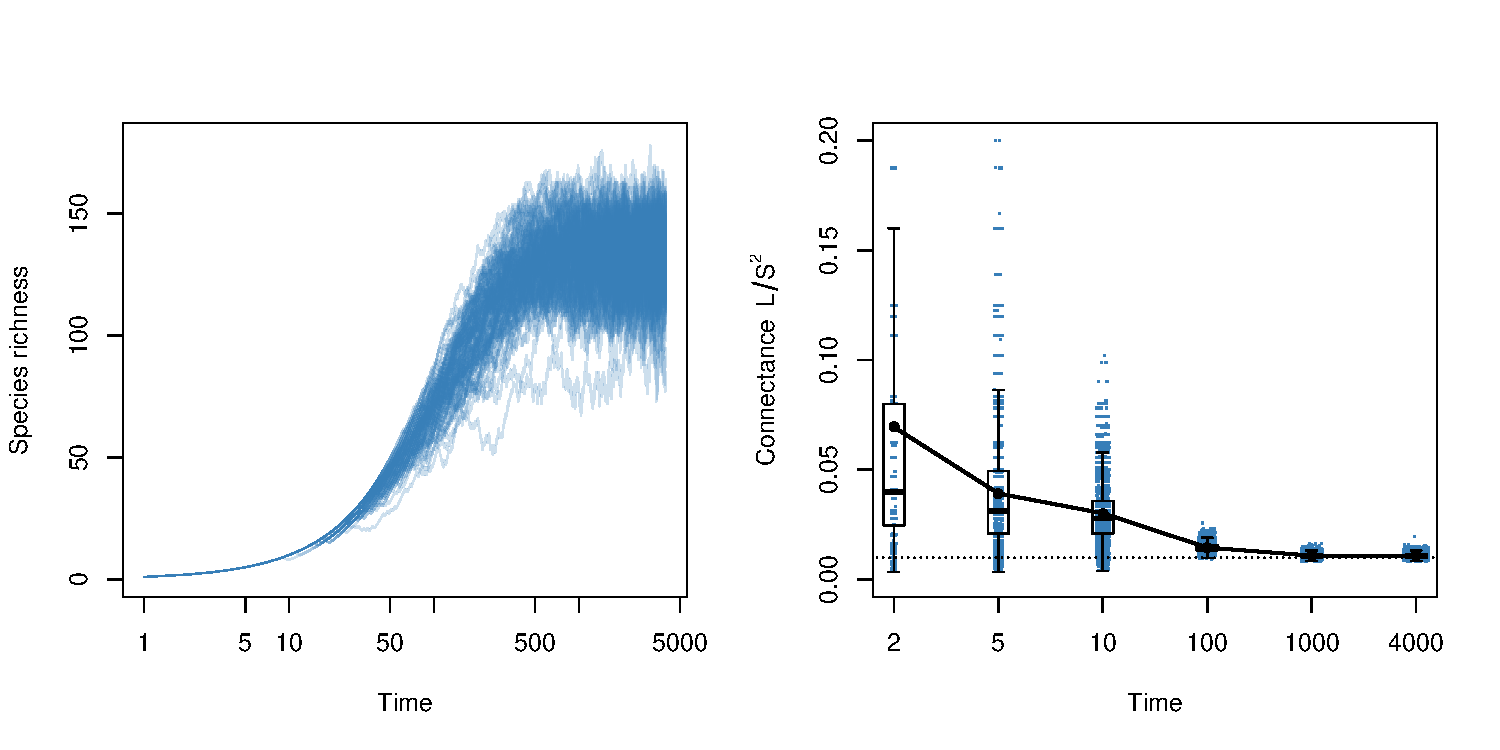
\includegraphics[width=0.8\textwidth]{fig_conn.pdf}
% \caption{
% A. Assembly of communities over time results in steady state species richness by ca. time-step 250.
% B. Trophic connectance early in assembly is high because few species are tightly connected.
% Over time, connectance decays as species richness increases, and the density of trophic interactions declines.
% }
% \label{fig:conn}
% \end{figure*}
% 
% 
% 
% \begin{figure*}[h!]
% \centering
% 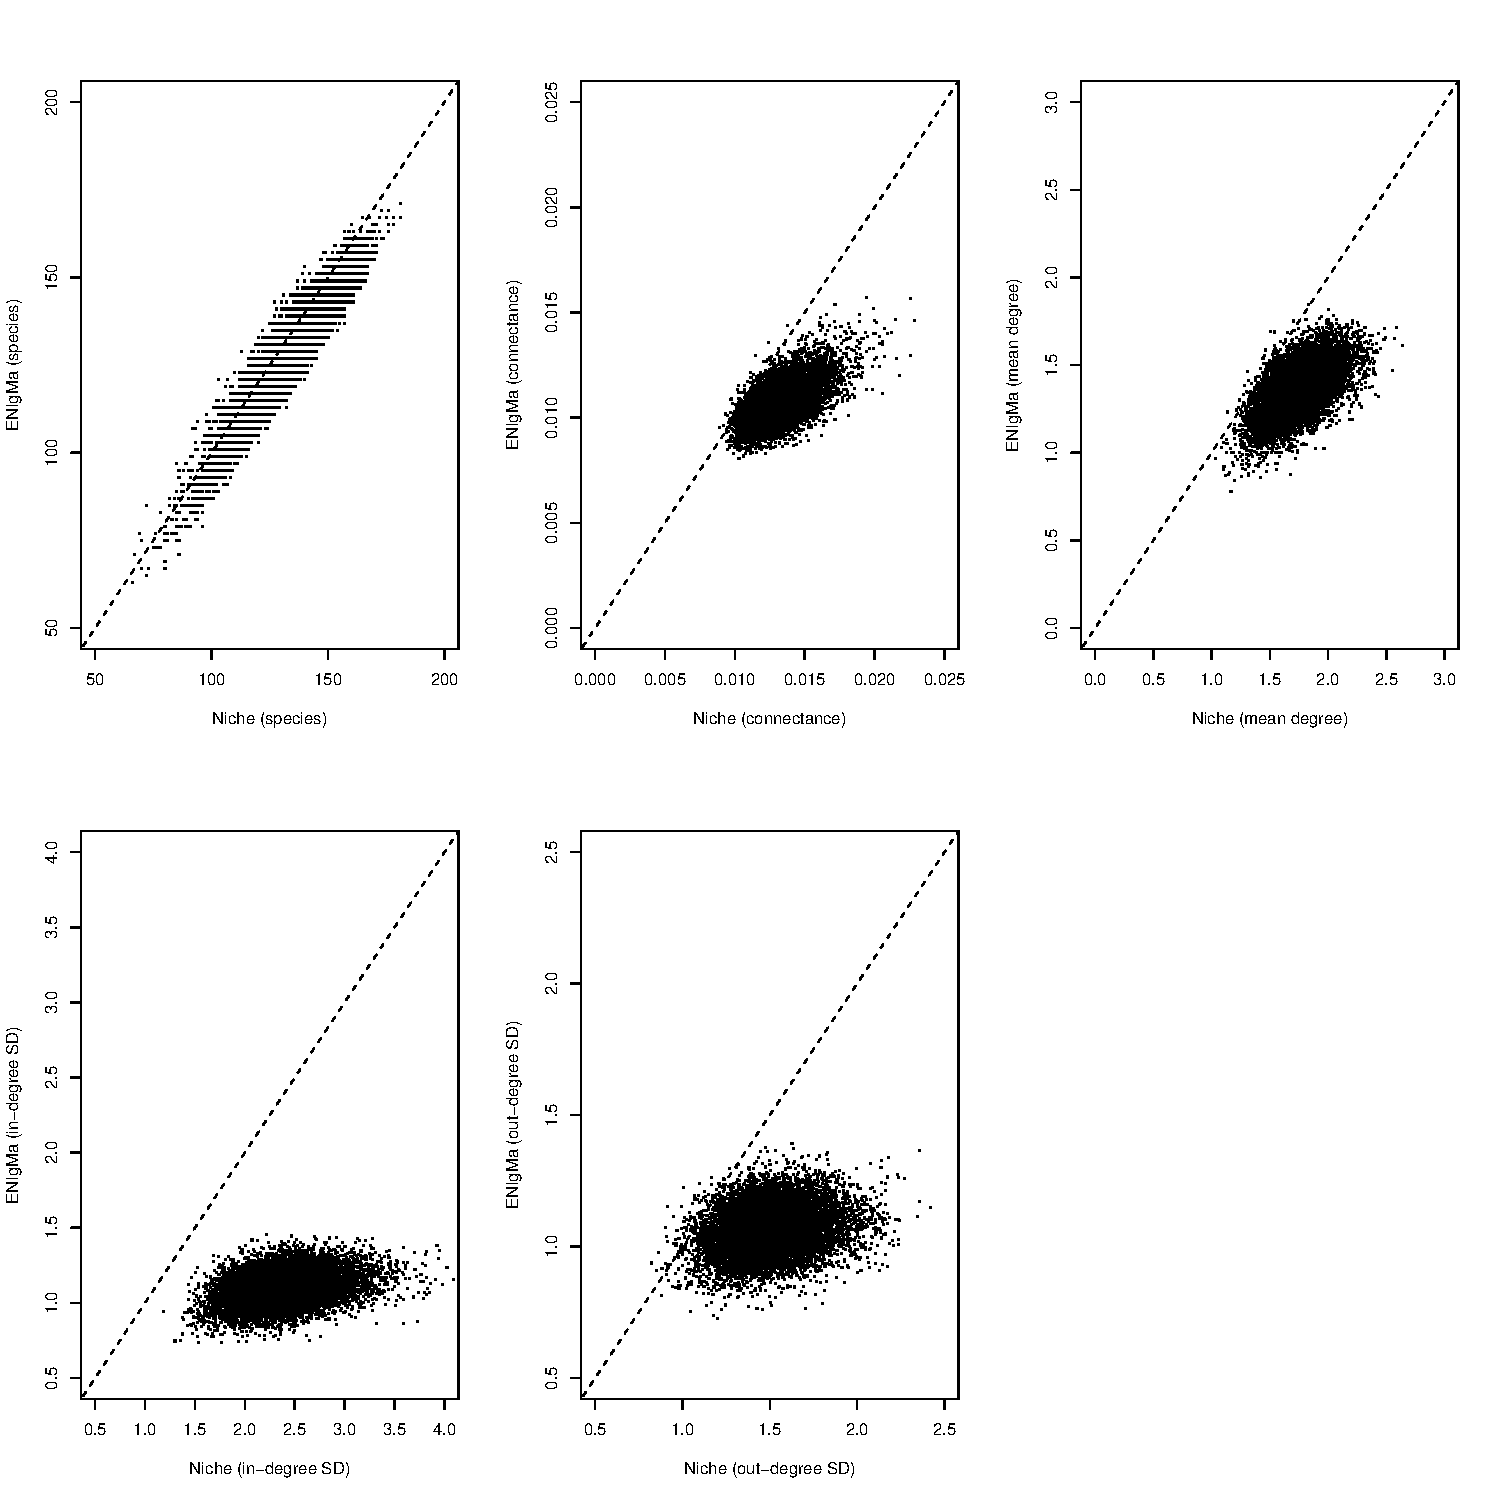
\includegraphics[width=0.8\textwidth]{fig_errorscatter.pdf}
% \caption{
% Comparisons of raw structural measures for the assembly (y-axis) and Niche model (x-axis).
% If the models produce similar structures, metrics will tend to fall on the 1:1 line (drawn).
% While the values for both models are similar, connectance, mean degree, and the standard deviation of in- and out-degree are all lower for the assembly model relative to those measures for the Niche model.
% }
% \label{fig:error1}
% \end{figure*}
% 
% \begin{figure*}[h!]
% \centering
% 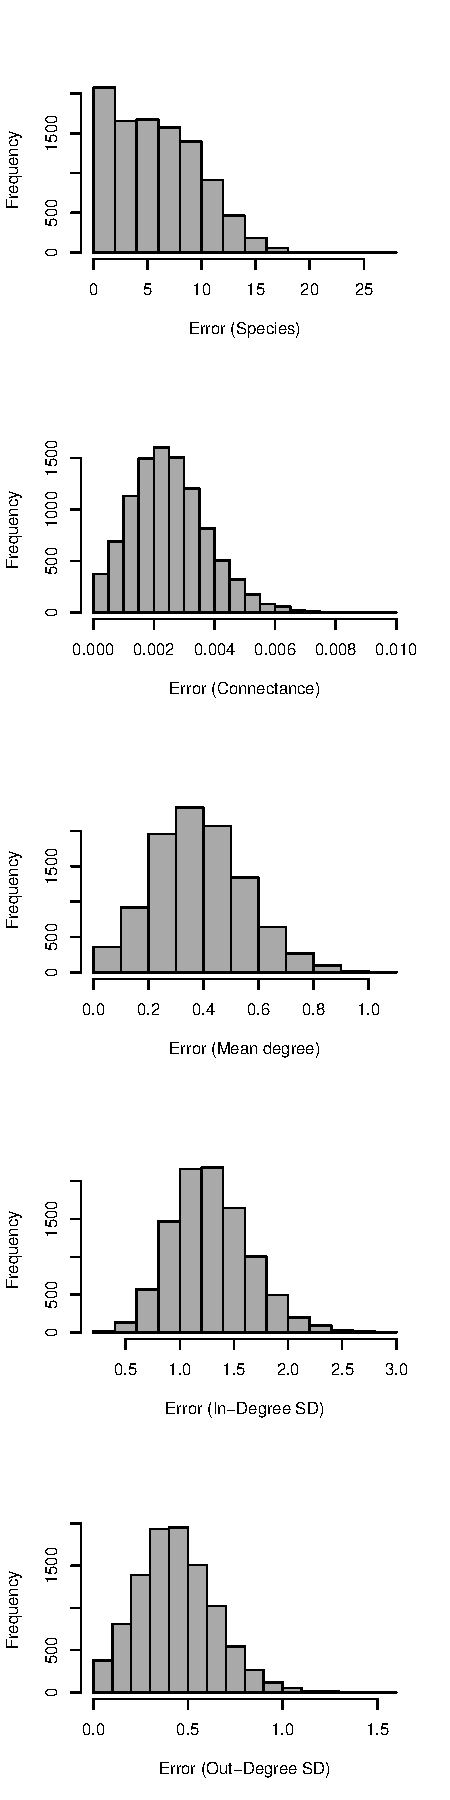
\includegraphics[width=0.3\textwidth]{fig_error.pdf}
% \caption{
% Error between structural measures of the assembly and Niche models.
% Error is measured as $\sqrt{(m_i - m_j)^2}$, where $m_i$ and $m_j$ are structural metrics for the assembly and Niche model, respectively.
% Only the trophic network of the assembly model used to assess metrics.
% }
% \label{fig:error2}
% \end{figure*}
% 
% \begin{figure*}[h!]
% \centering
% 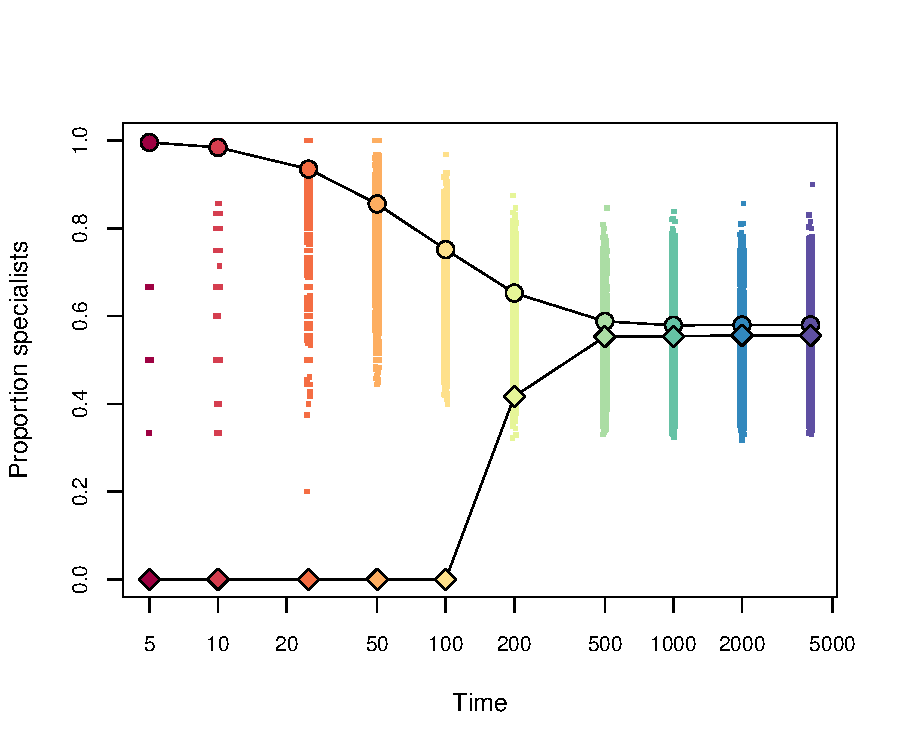
\includegraphics[width=0.8\textwidth]{fig_specialization.pdf}
% \caption{
% The proportion of specialists as a function of assembly time, where a specialist is defined as a species with a generality index $G_i < 1$.
% Measures of $G_i$ are shown normalized to different measures of link-density.
% Circles: $G_i^{\rr{all}}$ where $L$ accounts for all links in the food web and $S$ accounts for all species relative to each time interval in the assembly process (averaged across replicates).
% Points: $G_i^{\rr{hetero}}$, where we consider only the links and species richness of heterotrophs, excluding autotrophs (each point shows an individual replicate).
% Diamonds: $G_i^*$, where $L$ and $S$ are measured with respect to the communities at steady state (averaged across replicates). 
% This measure is the one presented in the main text and most similar to that used to evaluate assembling mangrove food webs \cite{Piechnik2008}.
% }
% \label{fig:spec}
% \end{figure*}
% 
% 
% 
% \begin{figure*}[h!]
% \centering
% 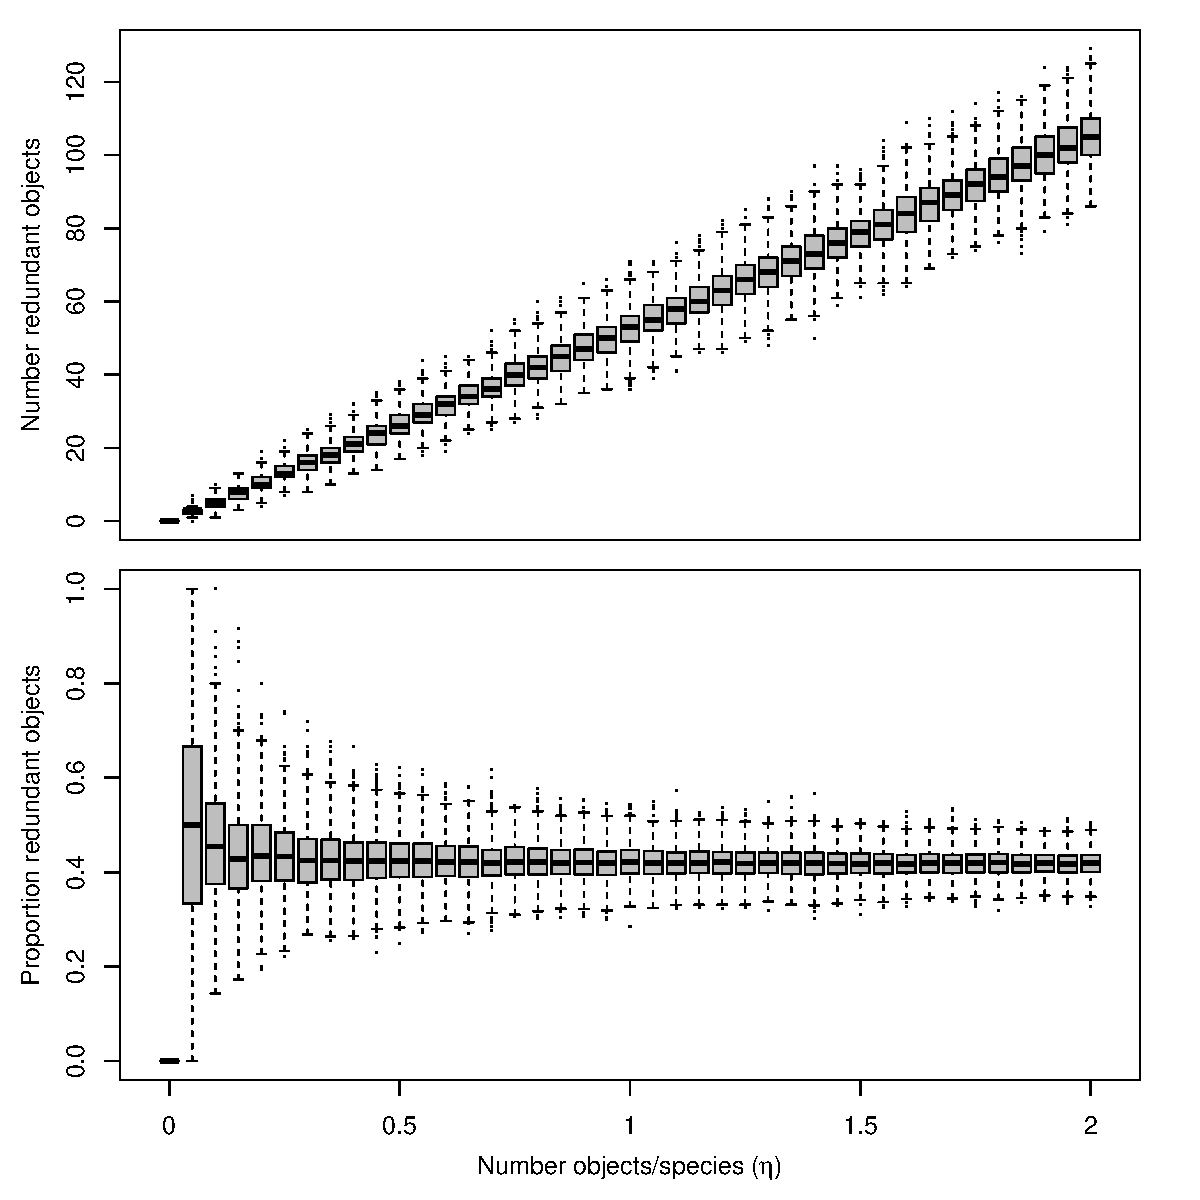
\includegraphics[width=0.8\textwidth]{fig_redundancy.pdf}
% \caption{
% A. Number of redundant modifiers in the source pool as a function of the expected number of modifiers made per species $\eta$.
% The red dashed line shows the analytical expectation (Eq. \ref{eq:redundant}).
% B. Proportion of redundant modifiers $\phi$ versus the total number of modifiers in the source pool as a function of the expected number of modifiers made per species $\eta$.
% The red dashed line shows the analytical expectation of $\phi \approx 0.418$ (Eq. \ref{eq:redundantprop}).
% }
% \label{fig:redundancy}
% \end{figure*}
% 
% \begin{figure*}[h!]
% \centering
% 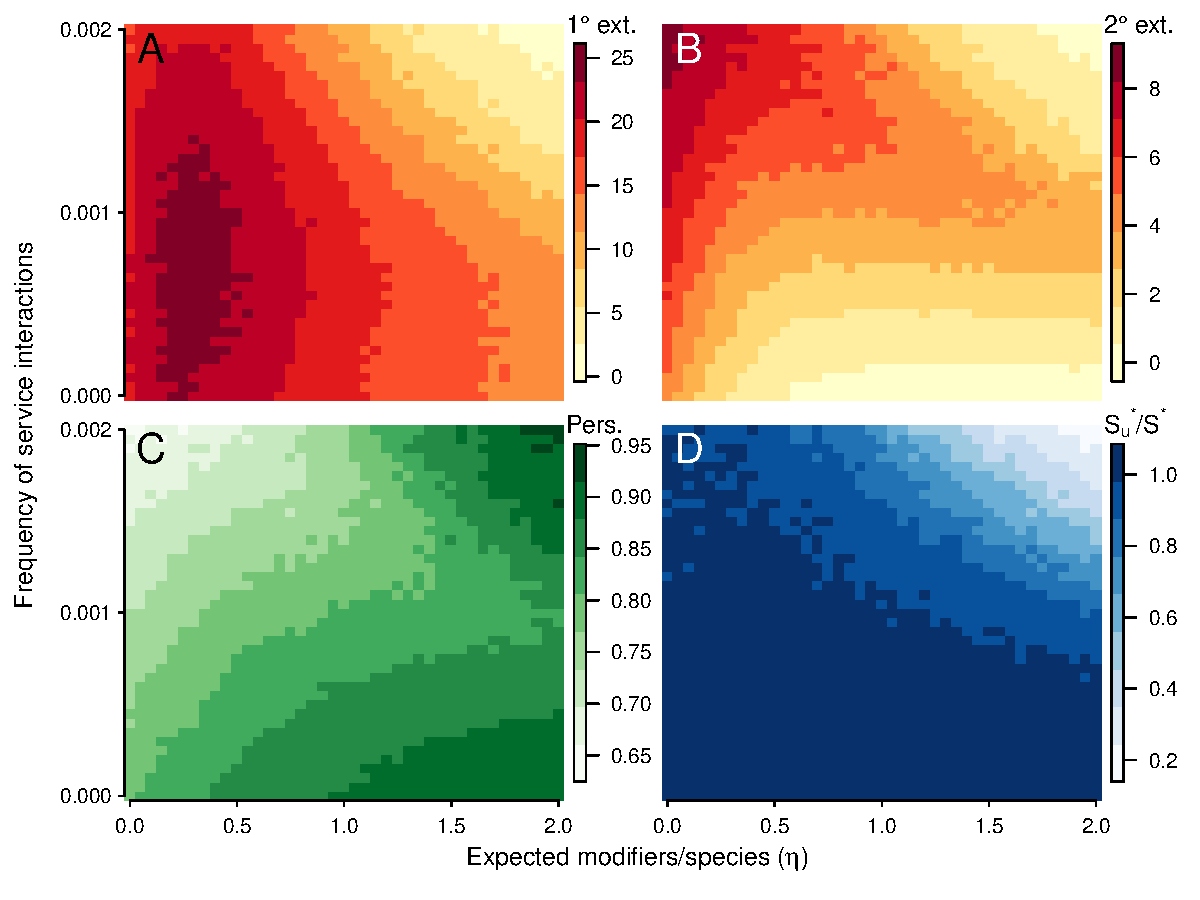
\includegraphics[width=0.8\textwidth]{fig_engineers4_unique.pdf}
% \caption{
% Measures of community robustness as a function of the frequency of service interactions and number of modifiers per species, where each modifier is uniquely made by an engineer.
% A. Mean rates of primary extinction, where primary extinctions occur from competitive exclusion of consumers over shared resources.
% B. Mean rates of secondary extinction, which cascade from primary extinctions.
% C. Mean species persistence, defined as the percent simulation time the community is occupied by a given species, averaged across all species that successfully colonize.
% D. The ratio $S^*_{\rm u}/S^*$, where $S^*_{\rm u}$ denotes steady states for systems where all engineered modifiers are unique to each engineer, and $S^*$ denote steady states for systems with redundant engineering. Lower values of $S^*_{\rm u}/S^*$ mean that systems with redundant engineers have higher steady states than those without redundancies.
% Values are averaged over 50 replicates for each parameterization.
% See Materials and Methods for default parameter values.
% }
% \label{fig:unique}
% \end{figure*}
% 
% \begin{figure*}[h!]
% \centering
% 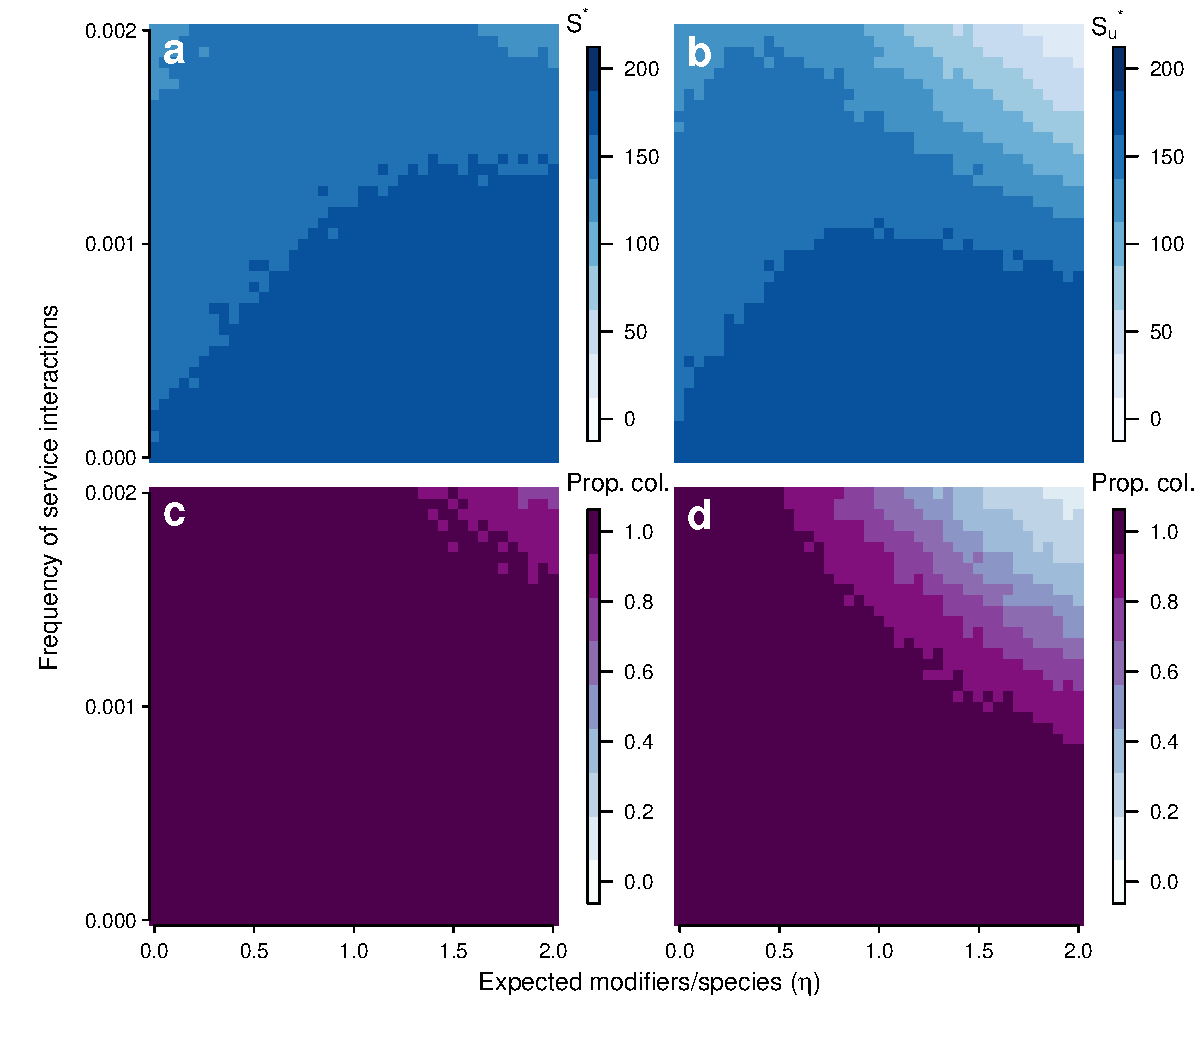
\includegraphics[width=0.8\textwidth]{fig_steadystates2.pdf}
% \caption{
% A. Steady state community richness with redundant engineering.
% B. Steady state community richness without redundant engineering.
% C. Proportion of species in the source pool that colonize the community at least once throughout the simulation (with redundant engineering).
% D. Proportion of species in the source pool that colonize the community at least once throughout the simulation (without redundant engineering).
% }
% \label{fig:steadystate}
% \end{figure*}


\end{document}
